\documentclass[10pt,aspectratio=169]{beamer}

\usetheme[numbering=fraction,progressbar=frametitle,block=fill]{metropolis}

\usepackage[T1]{fontenc}
\usepackage{amsmath,amssymb}
\usepackage{booktabs}
\usepackage{graphicx}
\usepackage{tikz}
\usepackage{circuitikz}
\usepackage{listings}
\usepackage{xcolor}
\usetikzlibrary{arrows.meta,positioning,fit,calc}

\graphicspath{{figures/}}

\definecolor{mDarkTeal}{HTML}{23373B}
\definecolor{mTeal}{HTML}{2D8A8A}
\definecolor{mGold}{HTML}{D6A13D}
\definecolor{mRed}{HTML}{B95050}
\definecolor{mGreen}{HTML}{4B8B5A}
\definecolor{mLight}{HTML}{F4F6F5}

\setbeamercolor{normal text}{fg=mDarkTeal,bg=white}
\setbeamercolor{alerted text}{fg=mRed}
\setbeamercolor{example text}{fg=mGreen}
\setbeamercolor{frametitle}{fg=white,bg=mDarkTeal}
\setbeamercolor{progress bar}{fg=mTeal,bg=mLight}
\setbeamercolor{title separator}{fg=mTeal}
\setbeamercolor{progress bar in head/foot}{fg=mTeal,bg=mLight}
\setbeamercolor{block title}{fg=white,bg=mDarkTeal}
\setbeamercolor{block body}{bg=mLight}

\setbeamertemplate{section in toc}[sections numbered]
\metroset{titleformat=smallcaps,sectionpage=none}

\newcommand{\proves}{\vdash}
\newcommand{\SC}{\mathrm{SC}}
\newcommand{\PoA}{\mathrm{PoA}}
\newcommand{\OPT}{\mathrm{OPT}}
\newcommand{\MMATPG}{\mathrm{MMATPG}}
\newcommand{\MATPG}{\mathrm{MATPG}}
\newcommand{\FRS}{\mathcal{FRS}}
\newcommand{\RS}{\mathcal{RS}}

\lstset{
  basicstyle=\ttfamily\scriptsize,
  breaklines=true,
  columns=fullflexible,
  keepspaces=true,
  frame=single,
  rulecolor=\color{mLight},
  backgroundcolor=\color{mLight},
  literate=
    {ℂ}{{$\mathbb{C}$}}1
    {ℝ}{{$\mathbb{R}$}}1
    {∀}{{$\forall$}}1
    {ᶠ}{{$^f$}}1
    {𝓝}{{$\mathcal{N}$}}1
    {∈}{{$\in$}}1
    {⊆}{{$\subseteq$}}1
    {ε}{{$\varepsilon$}}1
    {⟨}{{$\langle$}}1
    {⟩}{{$\rangle$}}1
    {∃}{{$\exists$}}1
    {→}{{$\to$}}1
    {↔}{{$\leftrightarrow$}}1
    {∧}{{$\wedge$}}1
    {≤}{{$\le$}}1
    {·}{{$\cdot$}}1
    {₀}{{$_0$}}1
    {₁}{{$_1$}}1
    {₂}{{$_2$}}1
    {₃}{{$_3$}}1
    {±}{{$\pm$}}1
}

\title{Multi-Agent Theorem Proving}
\subtitle{Allocation, Incentives, Markets, and Learning}
\author{Riyaz Ahuja}
\institute{Department of Mathematics, Carnegie Mellon University}
\date{Master's Thesis Defense \\ April 16, 2026}

\begin{document}

\maketitle

\section{Thesis}

\begin{frame}{The Core Claim}
\large
\begin{block}{Thesis}
Large-scale theorem proving is not just proof search. It is an allocation problem over interdependent proof obligations, distributed agents, private information, and incentives.
\end{block}

\vspace{0.8em}
\normalsize
\begin{itemize}
  \item A proof assistant verifies local correctness.
  \item A large formalization project still needs global coordination.
  \item The order of proving, conjecturing, and publishing results affects total project time.
  \item Markets and learning can coordinate decentralized agents without a central planner.
\end{itemize}
\end{frame}

\begin{frame}{Motivating Picture: PNT Dependencies}
\begin{columns}[T,onlytextwidth]
\column{0.52\textwidth}
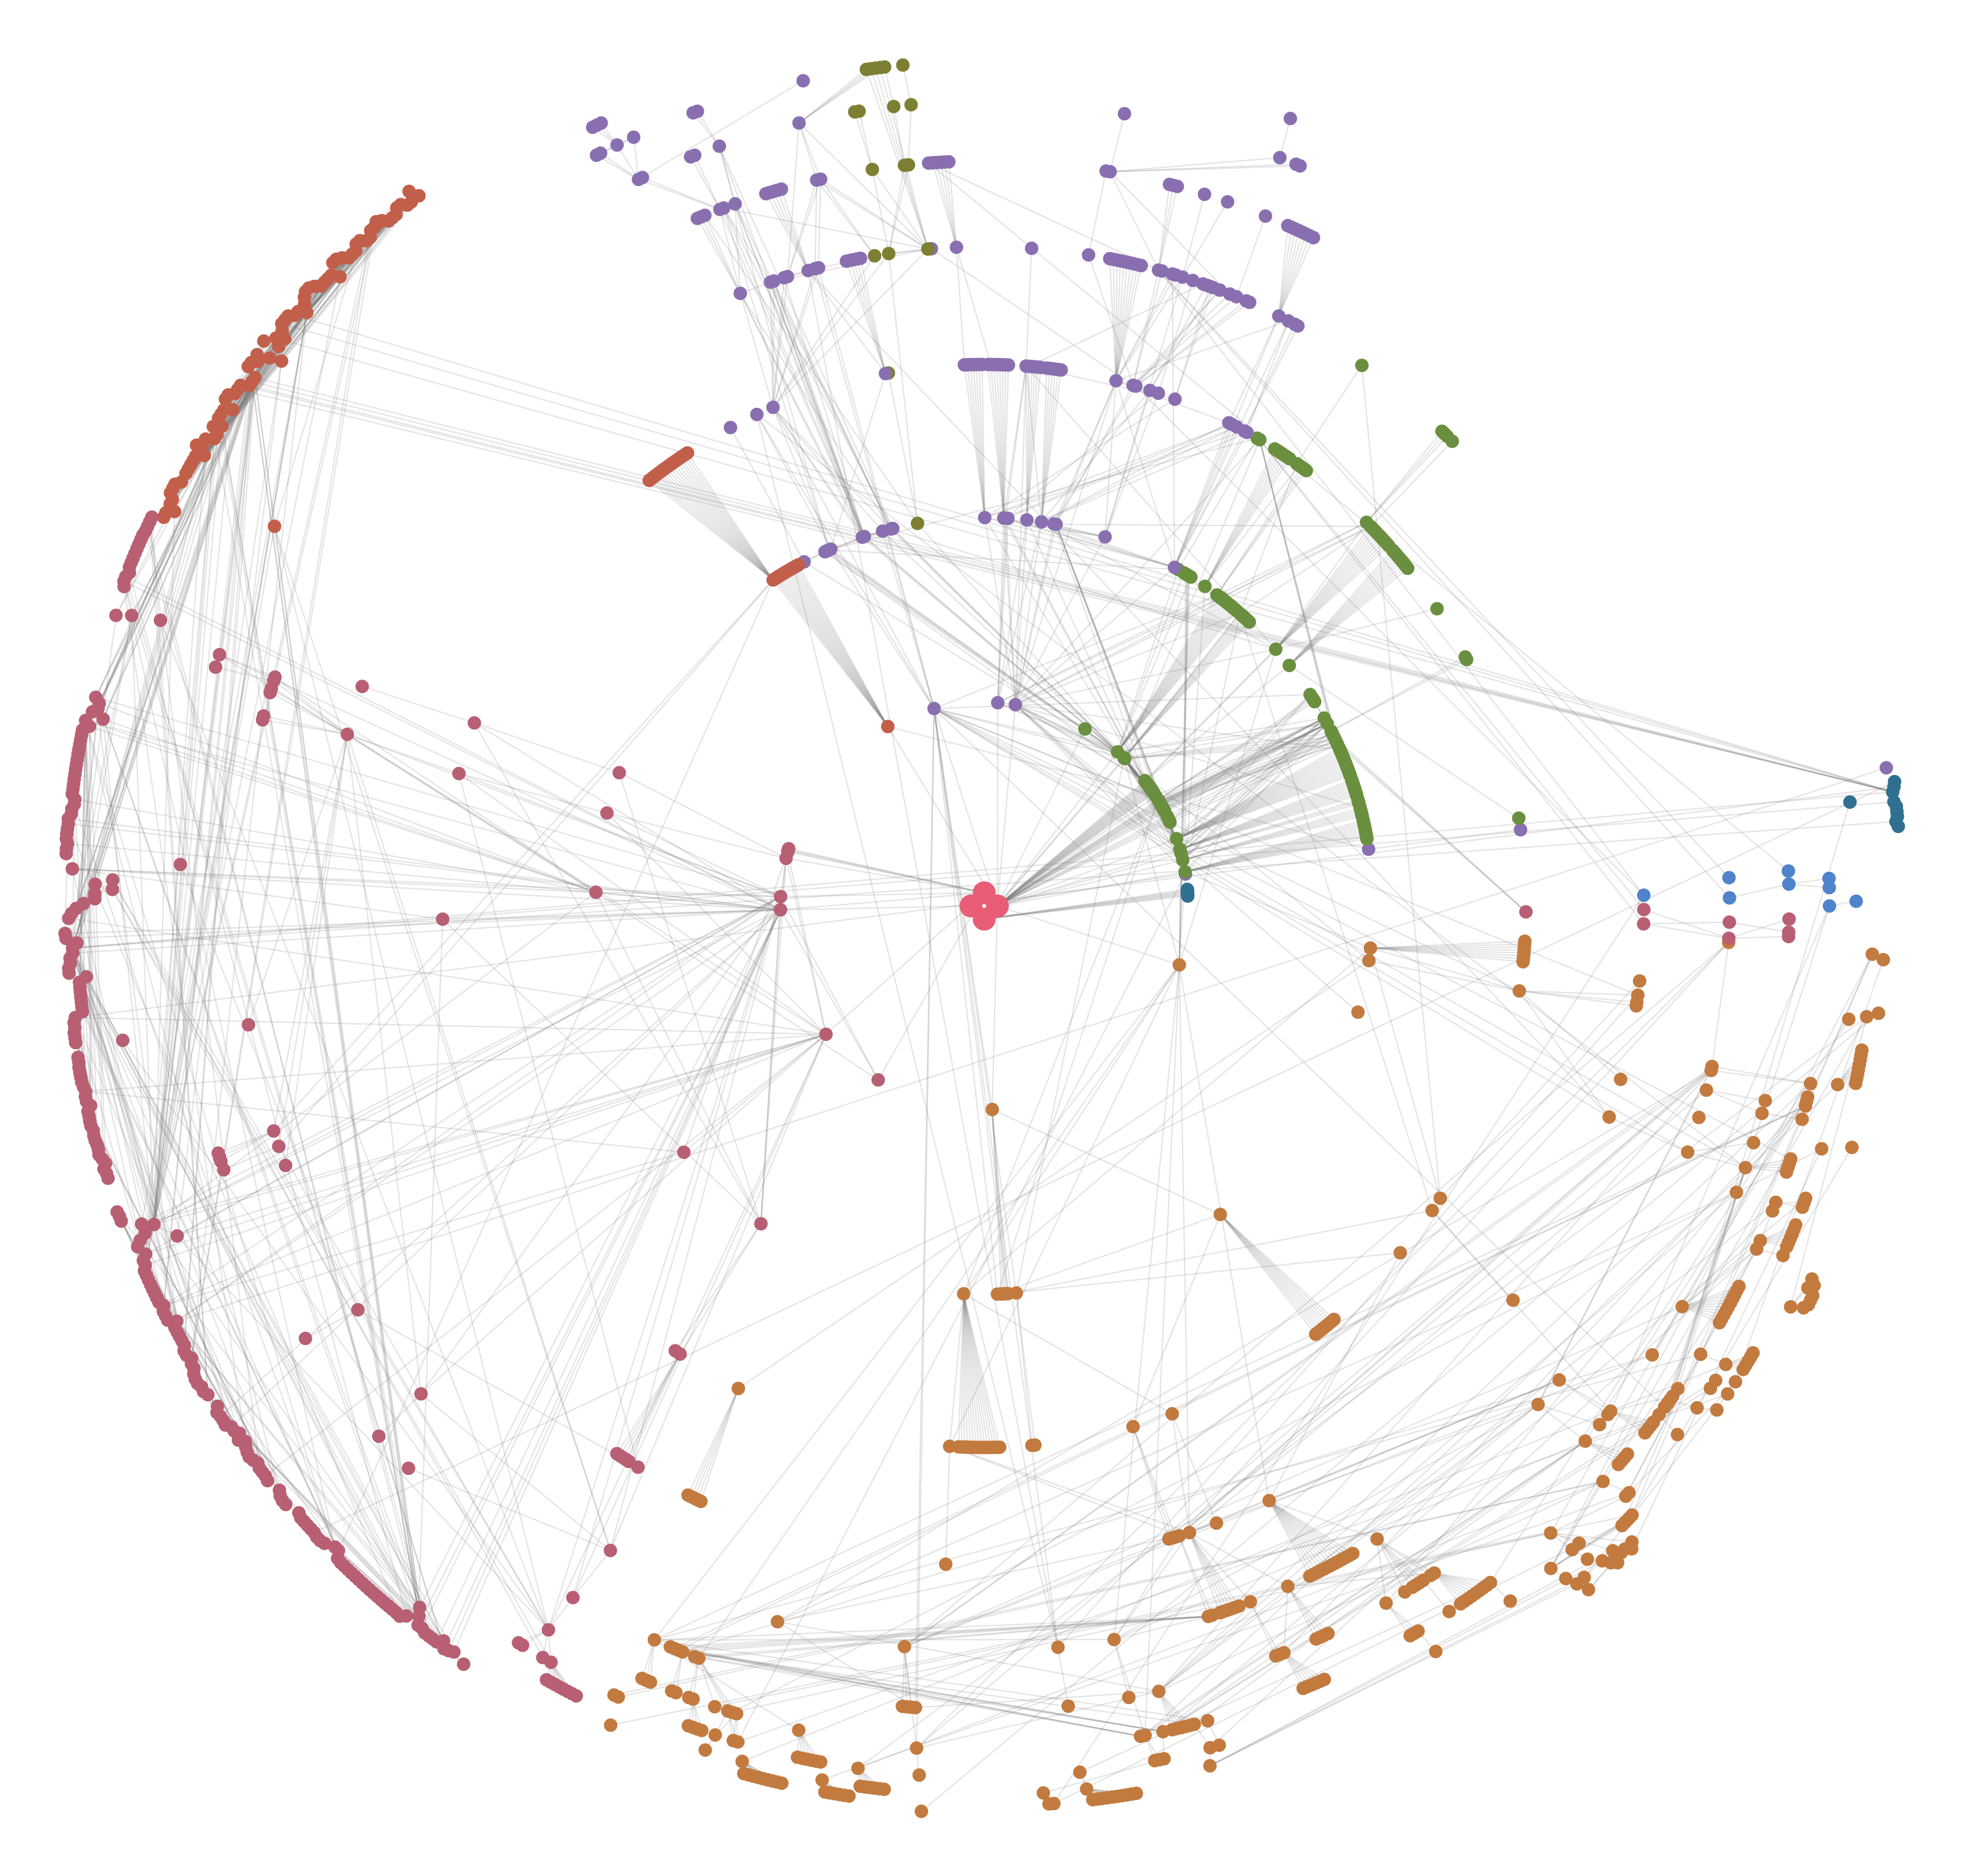
\includegraphics[width=\textwidth,height=0.72\textheight,keepaspectratio]{PNT_dependency.png}
\column{0.43\textwidth}
\small
\begin{itemize}
  \item The Prime Number Theorem is a final node in a large dependency network.
  \item Useful work is often indirect: lemmas, definitions, auxiliary infrastructure, and cross-domain tools.
  \item In Lean, this dependency structure becomes machine-visible.
  \item That makes coordination a formal object, not just a social practice.
\end{itemize}
\end{columns}
\end{frame}

\begin{frame}{Contributions in One Slide}
\small
\begin{tabular}{p{0.23\textwidth}p{0.67\textwidth}}
\toprule
\textbf{Area} & \textbf{Contribution} \\
\midrule
Formalism & Sequents, private/shared libraries, proof and conjecture kernels. \\
Centralized theory & PPI relaxation, NP-hardness, lower bounds, RLS $(2-1/m)$ approximation. \\
Game theory & MATPG, publication externality, unbounded PoA under credit rewards. \\
Mechanism design & MMATPG with bilateral contracts, market internalization, bounded PoA. \\
Learning & MAPPO + PSRO style population training with approximate CCE guarantees. \\
Systems & Agora scaffold with VerifiedAgora, markets, and LLM agents on Lean projects. \\
\bottomrule
\end{tabular}
\end{frame}

\section{Centralized MATP}

\begin{frame}{Mathematical Work Units}
\small
\begin{block}{Formula}
A statement $\phi$ in a formal language such as Lean, with negation $\neg\phi$.
\end{block}
\begin{block}{Sequent}
A proof obligation $[\Gamma \proves \phi]$: prove consequent $\phi$ from context $\Gamma$.
\end{block}
\begin{block}{Dependency}
A resolved sequent may depend on a finite set of formulas:
\[
\delta_t([\Gamma \proves \phi]) \subseteq \Gamma.
\]
\end{block}

\vspace{0.2em}
\centering
\textit{In the slides, think of formulas as nodes and sequents as targetable proof obligations.}
\end{frame}

\begin{frame}{Libraries Encode Mathematical State}
\small
At time $t$, a library is
\[
\mathcal{L}_t=(\mathcal{C}_t,\mathcal{RS}_t,\delta_t,\Theta_t).
\]

\begin{itemize}
  \item $\mathcal{C}_t$: concrete formulas that have been stated or conjectured.
  \item $\mathcal{RS}_t$: resolved sequents.
  \item $\delta_t$: dependency data for proofs.
  \item $\Theta_t$: solve-time and credited agent metadata.
\end{itemize}

\vspace{0.5em}
\begin{block}{Core invariants}
Libraries grow monotonically, proofs are dependency-acyclic, and public knowledge is included in every agent's private library.
\end{block}
\end{frame}

\begin{frame}{Full Resolution vs. Local Resolution}
\small
\begin{itemize}
  \item A proof can be locally resolved before all of its dependencies are themselves fully proved.
  \item $\RS_t$ records proof witnesses; $\FRS_t$ records proofs whose dependency closure is already resolved.
  \item This distinction is what makes intermediate lemmas valuable: a result may unlock downstream full resolution without being a final target.
\end{itemize}

\begin{block}{Inductive idea}
A sequent is fully resolved if it is an axiom, or every formula appearing in its dependency set has a fully resolved supporting sequent in the same context.
\end{block}
\end{frame}

\begin{frame}{Agent Action Primitives}
\small
\begin{tabular}{p{0.22\textwidth}p{0.68\textwidth}}
\toprule
\textbf{Action} & \textbf{Meaning} \\
\midrule
\texttt{Prove} & Allocate a time budget to a target sequent; success returns dependencies. \\
\texttt{Conj} & Propose a new formula or helper lemma. \\
\texttt{Pub} & Move private results into the shared library, with dependency closure. \\
\texttt{Qry} & Ask the agent's query model for success probability and expected duration. \\
\texttt{No-op} & Idle or forced idle while a durative job is running. \\
\bottomrule
\end{tabular}

\vspace{0.8em}
The proof and conjecture primitives are stochastic kernels; publication and query updates are deterministic bookkeeping.
\end{frame}

\begin{frame}{Centralized MATP as a POMDP}
\small
\begin{block}{Control problem}
A single planner allocates all agents across proof, conjecture, publication, and query actions.
\end{block}

\begin{itemize}
  \item Hidden state includes each agent's private library, jobs, query model, and cumulative effort.
  \item Observation is the public library plus recent query outputs.
  \item Cost counts unresolved targets:
  \[
  c(s_t,a_t)=\sum_{s\in\Phi^*}\mathbf{1}[s\notin \FRS^0_t].
  \]
  \item Makespan objective:
  \[
  C_{\max}=\inf\{t:\Phi^*\subseteq \FRS^0_t\}.
  \]
\end{itemize}
\end{frame}

\begin{frame}{Centralized Transition: What Happens in One Step}
\small
\begin{enumerate}
  \item \textbf{Pre-update:} decrement active job timers; start new proof/conjecture jobs for idle agents; apply publications; refresh query buffers.
  \item \textbf{Stochastic completion:} each job whose timer hits zero draws from the relevant proof or conjecture kernel.
  \item \textbf{Post-update:} successful proofs add resolved sequents and dependency data; successful conjectures add new concrete formulas; completed jobs clear.
\end{enumerate}

\begin{block}{Reason for the formal machinery}
It separates the physics of proof attempts from the planner's information problem. The same transition dynamics will later be reused in the decentralized game.
\end{block}
\end{frame}

\begin{frame}{Perfect Public Information Relaxation}
\small
\begin{block}{Theorem}
Let $\OPT$ be the optimal expected makespan in the full centralized model, and $\OPT_{\mathrm{PPI}}$ under perfect public information. Then
\[
\OPT_{\mathrm{PPI}}\le \OPT.
\]
\end{block}

\begin{itemize}
  \item PPI makes every proof immediately public.
  \item The planner observes the full state instead of a belief over private libraries.
  \item This is a lower-bound and hardness-friendly relaxation.
  \item It gives a clean scheduling-theoretic core.
\end{itemize}
\end{frame}

\begin{frame}{Proof Idea: PPI Is a Relaxation}
\small
\begin{enumerate}
  \item In the original model, proof results first live in private libraries and require an explicit publication action.
  \item In PPI, every proof completion is immediately public, so publication costs disappear.
  \item In the original model, the planner observes only the public projection and query outputs.
  \item In PPI, the planner sees the full state. More information cannot hurt an optimal controller.
\end{enumerate}

\begin{block}{Consequence}
Any lower bound or hardness result for PPI also applies to the full centralized problem.
\end{block}
\end{frame}

\begin{frame}{The Revelation DAG}
\small
\begin{block}{Non-conjecturing PPI MATP}
All formulas are already concrete, and the only unknown is which dependencies will be revealed when a target is solved.
\end{block}

\begin{itemize}
  \item Latent task set: $\mathcal{T}^*=\mathrm{cl}(\Phi^*)$.
  \item Revelation DAG: $s\to s'$ when solving $s$ reveals that $s'$ is required.
  \item There is no operational precedence: an agent may attempt any concrete sequent.
  \item The bottleneck is informational: the planner may not know which tasks matter yet.
\end{itemize}
\end{frame}

\begin{frame}{Example: Informational Precedence}
\small
\begin{center}
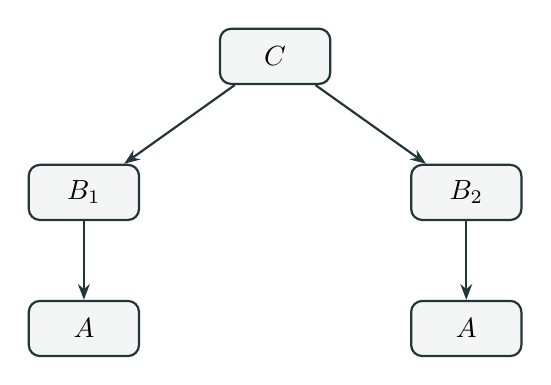
\begin{tikzpicture}[
  node/.style={draw=mDarkTeal,thick,rounded corners,fill=mLight,minimum width=1.4cm,minimum height=0.7cm,align=center},
  arr/.style={-{Stealth[length=2mm]},thick,mDarkTeal}
]
\node[node] (c) {$C$};
\node[node,below left=1.0cm and 1.0cm of c] (b1) {$B_1$};
\node[node,below right=1.0cm and 1.0cm of c] (b2) {$B_2$};
\node[node,below=1.0cm of b1] (a1) {$A$};
\node[node,below=1.0cm of b2] (a2) {$A$};
\draw[arr] (c) -- (b1);
\draw[arr] (c) -- (b2);
\draw[arr] (b1) -- (a1);
\draw[arr] (b2) -- (a2);
\end{tikzpicture}
\end{center}

\small
The planner may attempt $B_1$ or $B_2$ before proving $C$, but it does not know they matter until resolving $C$ reveals its dependencies.
\end{frame}

\begin{frame}{Lower Bounds: Work and Serial Depth}
\small
For a realization $\omega$:
\[
W(\omega)=\sum_{s\in\mathcal{T}^*}\min_\alpha T^\alpha_s(\omega),
\qquad
D(\omega)=\max_{\text{chain}}\sum_{s\in\text{chain}}\min_\alpha T^\alpha_s(\omega).
\]

\begin{block}{Theorem}
For any policy $\pi$,
\[
\mathbb{E}^\pi[C_{\max}]\ge
\max\left\{\frac{\mathbb{E}[W]}{m},\mathbb{E}[D]\right\}.
\]
\end{block}

\begin{itemize}
  \item $W/m$: even perfect parallelism cannot process less total work.
  \item $D$: latent dependency chains impose serial discovery.
\end{itemize}
\end{frame}

\begin{frame}{Proof Sketch: Lower Bounds}
\small
\begin{block}{Work bound}
Every task in $\mathcal{T}^*$ must eventually be resolved. Even with perfect scheduling, $m$ agents can process at most $m$ units of work per unit time:
\[
C_{\max}(\omega)\ge W(\omega)/m.
\]
\end{block}

\begin{block}{Serial-depth bound}
On any revelation chain $s_0\to s_1\to\cdots\to s_k$, task $s_{i+1}$ is not known to be required until $s_i$ resolves. The chain therefore forces at least
\[
\sum_i \min_\alpha T^\alpha_{s_i}(\omega)
\]
time, unless speculation has already resolved a link; in that case its realized remaining time is zero.
\end{block}
\end{frame}

\begin{frame}{Centralized Hardness}
\small
\begin{block}{Theorem}
The non-conjecturing PPI MATP decision problem is NP-hard, even with identical agents, deterministic proof kernels, and trivial dependencies.
\end{block}

\begin{itemize}
  \item Reduction from makespan minimization on identical parallel machines.
  \item Under PPI, the problem is an MDP and lies in PSPACE for finite horizons.
  \item The state space is exponential because the resolved set ranges over subsets of tasks.
  \item Conjecturing makes the task space endogenous and harder.
\end{itemize}
\end{frame}

\begin{frame}{Proof Sketch: NP-Hardness}
\small
\begin{itemize}
  \item Reduce from $P\|C_{\max}$: schedule jobs on identical parallel machines.
  \item Create one sequent $s_j$ for each job $j$, with deterministic proof time $p_j$.
  \item Use $m$ identical agents as the $m$ machines.
  \item Set $\delta^*(s_j)=\varnothing$, so every resolved sequent is immediately fully resolved.
  \item The MATP makespan equals the machine-scheduling makespan exactly.
\end{itemize}

\begin{block}{Why this matters}
The hardness is present before conjecturing, private information, strategic behavior, or markets are added.
\end{block}
\end{frame}

\begin{frame}{Reactive List Scheduling}
\small
\begin{block}{RLS policy}
\begin{enumerate}
  \item Initialize a known task queue with $\Phi^*$.
  \item Assign idle agents to highest-priority unresolved known tasks.
  \item When a proof completes, add newly revealed dependencies to the queue.
\end{enumerate}
\end{block}

\begin{itemize}
  \item Priority function can be arbitrary for the worst-case guarantee.
  \item A redundant variant sends extra agents to the same unresolved task when the queue is narrow.
  \item This is the theorem-proving analogue of list scheduling under latent precedence.
\end{itemize}
\end{frame}

\begin{frame}{RLS Algorithm Walkthrough}
\small
\begin{block}{State maintained by scheduler}
\[
\mathcal{K}_t=\text{known unresolved tasks}
\]
initialized with the target set $\Phi^*$ and expanded whenever a proof reveals new dependencies.
\end{block}

\begin{enumerate}
  \item Rank $\mathcal{K}_t\setminus\RS^0_t$ by priority $\sigma$.
  \item Assign idle agents to the best currently unassigned known tasks.
  \item If the known queue is narrow, optional redundant RLS sends extra agents to the same bottleneck task.
  \item On resolution of $s$, add the sequents induced by $\delta^*(s)$ to $\mathcal{K}_{t+1}$.
\end{enumerate}
\end{frame}

\begin{frame}{RLS Approximation Guarantee}
\small
\begin{block}{Theorem}
For identical agents and single-assignment RLS:
\[
C_{\max}^{\mathrm{RLS}}(\omega)
\le
\frac{W(\omega)}{m}+\left(1-\frac{1}{m}\right)D(\omega).
\]
Therefore
\[
\mathbb{E}[C_{\max}^{\mathrm{RLS}}]\le
\left(2-\frac{1}{m}\right)\mathbb{E}[\OPT].
\]
\end{block}

\begin{itemize}
  \item Busy time is controlled by total work.
  \item Starved time is charged to a revelation chain.
  \item The guarantee matches Graham-style scheduling intuition.
\end{itemize}
\end{frame}

\begin{frame}{Proof Sketch: RLS Approximation}
\small
\begin{enumerate}
  \item Let $s^*$ be the last task completed by RLS.
  \item Split time before $C_{s^*}$ into \textbf{busy} intervals, where all agents work, and \textbf{starved} intervals, where at least one agent is idle.
  \item Busy intervals consume total work, so
  \[
  B\le W/m.
  \]
  \item Starved intervals happen only while waiting along a revelation chain ending at $s^*$, so their excess cost is bounded by
  \[
  \left(1-\frac1m\right)D.
  \]
  \item Combine with $\OPT\ge \max\{W/m,D\}$.
\end{enumerate}
\end{frame}

\begin{frame}{Redundancy on Narrow Chains}
\small
\begin{block}{Proposition}
For a pure revelation chain $s_0\to s_1\to\cdots\to s_k$ with i.i.d. $\mathrm{Exp}(\lambda)$ task times:
\[
\mathbb{E}[C_{\max}^{\mathrm{single}}]=(k+1)/\lambda,
\qquad
\mathbb{E}[C_{\max}^{\mathrm{redundant}}]=(k+1)/(m\lambda).
\]
\end{block}

\begin{itemize}
  \item Single-assignment RLS waits for one exponential clock per chain node.
  \item Redundant RLS runs $m$ independent clocks; the minimum is $\mathrm{Exp}(m\lambda)$.
  \item This motivates learned OR-parallelism on bottleneck targets.
\end{itemize}
\end{frame}

\begin{frame}{Why Centralization Is Not Enough}
\small
The centralized model gives a benchmark, but it assumes too much.

\begin{itemize}
  \item Agents control their own compute.
  \item Agents have private search state and local discoveries.
  \item Publication is optional and costly.
  \item Credit, reputation, market value, and opportunity cost are individual incentives.
\end{itemize}

\begin{block}{Next question}
Can independent agents achieve centralized-like efficiency without a planner?
\end{block}
\end{frame}

\section{Markets and Decentralization}

\begin{frame}{From POMDP to POSG}
\small
\begin{block}{MATPG}
The Multi-Agent Theorem Proving Game uses the same proof environment as centralized MATP, but each agent chooses its own action from its own observation history.
\end{block}

\begin{itemize}
  \item State and transition dynamics are unchanged.
  \item Agent $\alpha$ observes its private library, query responses, and the public library.
  \item Other agents' private libraries and job states are hidden.
  \item Rewards are individual, not a shared social objective.
\end{itemize}
\end{frame}

\begin{frame}{Efficiency Metric}
\small
Social cost is expected time until all public targets are fully resolved:
\[
\SC(\pi)=\mathbb{E}^{\pi}\left[\inf\{t\ge0:\Phi^*\subseteq\FRS^0_t\}\right].
\]

\begin{block}{Price of Anarchy}
\[
\PoA=\frac{\sup_{\pi^*\in\mathrm{NE}}\SC(\pi^*)}{\inf_{\pi}\SC(\pi)}.
\]
\end{block}

\begin{itemize}
  \item $\PoA=1$: equilibria are socially optimal.
  \item Large $\PoA$: decentralization creates serious inefficiency.
  \item Infinite $\PoA$: some equilibria never finish the project.
\end{itemize}
\end{frame}

\begin{frame}{Credit-Based Rewards}
\small
\begin{block}{Reward}
Agent $\alpha$ earns value for newly public, fully resolved sequents credited to $\alpha$:
\[
r^\alpha_{\mathrm{credit}}(s_t,a_t)=
\sum_{s\in\FRS^0_{t+1}\setminus\FRS^0_t}
v(s)\mathbf{1}[\Theta^0_{t+1}(s)=(\cdot,\alpha)].
\]
\end{block}

\begin{itemize}
  \item This models priority and attribution.
  \item It is natural, but it rewards credited outputs, not the social value of enabling others.
  \item Byproduct lemmas can become privately useful but publicly underprovided.
\end{itemize}
\end{frame}

\begin{frame}{Publication Externality}
\small
\begin{block}{Definition}
A publication externality exists when publishing helps another agent but does not help the publisher.
\end{block}

\begin{itemize}
  \item Agent $\alpha$ privately proves a lemma $s_\alpha$.
  \item Agent $\beta$ needs $s_\alpha$ to complete a valuable target.
  \item Publishing $s_\alpha$ costs $\alpha$ time and may help a competitor.
  \item Under credit rewards, $\alpha$ may rationally withhold it.
\end{itemize}

\begin{block}{Theorem}
With at least two agents and nontrivial cross-agent dependencies, publication externalities exist.
\end{block}
\end{frame}

\begin{frame}{Proof Sketch: Publication Externality}
\small
\begin{columns}[T,onlytextwidth]
\column{0.48\textwidth}
\begin{block}{Construction}
\begin{itemize}
  \item $\alpha$ privately proves a byproduct $s_\alpha$.
  \item $v_\alpha(s_\alpha)=0$, so $\alpha$ gets no direct credit.
  \item $\beta$ needs $s_\alpha$ to finish valuable target $s_\beta$.
\end{itemize}
\end{block}
\column{0.48\textwidth}
\begin{block}{Payoff comparison}
\begin{itemize}
  \item Publishing costs $\alpha$ a timestep and may help a competitor.
  \item Publishing strictly improves $\beta$'s future return.
  \item Therefore private and social incentives diverge.
\end{itemize}
\end{block}
\end{columns}

\vspace{0.6em}
\centering
\textit{The problem is not that agents fail to prove useful work; it is that useful work can remain private.}
\end{frame}

\begin{frame}{Unbounded PoA Without a Market}
\small
\begin{block}{Theorem}
The MATPG with credit-based rewards has unbounded Price of Anarchy.
\end{block}

\begin{itemize}
  \item Construct a dependency chain where each link is a byproduct of a different agent's private work.
  \item No agent is paid for publishing its byproduct.
  \item In a worst-case equilibrium, the public chain never completes.
  \item The centralized planner would simply instruct agents to publish.
\end{itemize}
\end{frame}

\begin{frame}{Proof Sketch: Unbounded PoA}
\small
\begin{center}
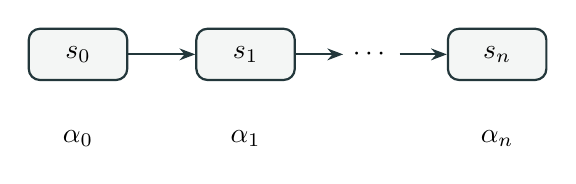
\begin{tikzpicture}[
  node/.style={draw=mDarkTeal,thick,rounded corners,fill=mLight,minimum width=1.25cm,minimum height=0.65cm,align=center},
  arr/.style={-{Stealth[length=2mm]},thick,mDarkTeal}
]
\node[node] (s0) {$s_0$};
\node[node,right=0.85cm of s0] (s1) {$s_1$};
\node[right=0.6cm of s1] (dots) {$\cdots$};
\node[node,right=0.6cm of dots] (sn) {$s_n$};
\draw[arr] (s0) -- (s1);
\draw[arr] (s1) -- (dots);
\draw[arr] (dots) -- (sn);
\node[below=0.5cm of s0] {$\alpha_0$};
\node[below=0.5cm of s1] {$\alpha_1$};
\node[below=0.5cm of sn] {$\alpha_n$};
\end{tikzpicture}
\end{center}

\small
\begin{itemize}
  \item Social target is $s_0$, but it requires a chain of byproducts.
  \item Each $s_i$ is privately available to a different agent as a zero-credit byproduct.
  \item No individual agent wants to pay the publication cost for its link.
  \item The centralized optimum publishes the chain; the worst equilibrium never resolves $s_0$.
\end{itemize}
\end{frame}

\begin{frame}{Market Idea}
\small
\begin{block}{Goal}
Turn the public resolution of a sequent into a tradable, verifiable economic event.
\end{block}

\begin{itemize}
  \item Agents who need a result can express demand.
  \item Agents who can provide it can buy exposure, prove it, publish it, and collect.
  \item Settlement depends on the shared library, so private hoarding does not pay.
  \item The proof assistant supplies the event oracle.
\end{itemize}
\end{frame}

\begin{frame}{Contract Mechanics by Example}
\small
Suppose $\chi=(s,T,\ell)$ with $\ell=0.1$.

\begin{tabular}{p{0.3\textwidth}p{0.28\textwidth}p{0.28\textwidth}}
\toprule
Outcome at $T$ & Long $\chi^+$ & Short $\chi^-$ \\
\midrule
$s$ is public & $+0.9$ & $-0.9$ \\
$s$ is not public & $-0.1$ & $+0.1$ \\
\bottomrule
\end{tabular}

\vspace{1em}
\begin{itemize}
  \item A beneficiary buys long exposure because it wants $s$ resolved.
  \item A prover buys long exposure because it can make the event true.
  \item A skeptic or hedger may take the short side.
  \item Collateral forces every participant to cover the worst-case loss.
\end{itemize}
\end{frame}

\begin{frame}{Collateralized Bilateral Contracts}
\small
A contract type is
\[
\chi=(s,T,\ell),
\]
a unit-notional claim on the event $E_{s,T}=1[s\in\RS^0_T]$.

\begin{columns}[T,onlytextwidth]
\column{0.48\textwidth}
\begin{block}{Long payoff}
\[
\Pi(\chi^+)=
\begin{cases}
1-\ell,& E_{s,T}=1,\\
-\ell,& E_{s,T}=0.
\end{cases}
\]
\end{block}
\column{0.48\textwidth}
\begin{block}{Short payoff}
\[
\Pi(\chi^-)=-\Pi(\chi^+).
\]
\end{block}
\end{columns}

\vspace{0.4em}
Positions are fully collateralized, so settlement cannot default.
\end{frame}

\begin{frame}{Market-Mediated MATPG}
\small
\begin{block}{MMATPG}
The MMATPG augments the MATPG world state with portfolios and a public order book.
\end{block}

\begin{itemize}
  \item Actions add posting offers, accepting offers, and issuing matched contract pairs.
  \item Observations add the agent's portfolio and the public ledger.
  \item Rewards are balance changes:
  \[
  r^\alpha_{\mathrm{mkt}}(w_t,a_t)=B^\alpha_{t+1}-B^\alpha_t.
  \]
  \item Contract settlement is triggered by public, verified Lean resolution.
\end{itemize}
\end{frame}

\begin{frame}{Internalizing the Externality}
\small
\begin{block}{Theorem}
If $\beta$ values public resolution of $s$ and $\alpha$ can resolve it at cost $c_\alpha$, contracts allow value to move from beneficiary to provider.
\end{block}

\begin{itemize}
  \item $\beta$ buys long exposure because $s$ being resolved helps its own goals.
  \item $\alpha$ buys or creates long exposure, proves $s$, publishes it, and collects settlement.
  \item The payoff requires $s\in\RS^0_T$, so publication is part of the incentive.
  \item The externality becomes a private profit opportunity.
\end{itemize}
\end{frame}

\begin{frame}{Proof Sketch: Market Internalization}
\small
\begin{enumerate}
  \item Agent $\beta$ values public resolution of $s$ by time $T$ at $v_\beta$.
  \item Agent $\alpha$ can resolve and publish $s$ at cost $c_\alpha$.
  \item If $\alpha$ can obtain $q$ long contracts at price $p$, then proving and publishing gives net payoff
  \[
  q(1-\ell)-qp-c_\alpha.
  \]
  \item This is profitable whenever
  \[
  q(1-\ell-p)>c_\alpha.
  \]
  \item Settlement checks $s\in\RS^0_T$, so private proof without publication does not collect.
\end{enumerate}
\end{frame}

\begin{frame}{Bounded PoA With the Market}
\small
\begin{block}{Theorem}
Under sufficient liquidity, resolvability, and positive gains from trade:
\[
\PoA \le \frac{1}{1-\ell}\left(2-\frac{1}{m}\right).
\]
\end{block}

\begin{itemize}
  \item The $(2-1/m)$ term is the centralized RLS scheduling factor.
  \item The $1/(1-\ell)$ term is market friction from contract downside.
  \item As $\ell\to0$, the market approaches a pure bounty system and recovers the RLS bound.
\end{itemize}
\end{frame}

\begin{frame}{Proof Sketch: Bounded PoA}
\small
\begin{enumerate}
  \item \textbf{No unresolved profitable task at equilibrium.} If $s\in\mathcal{T}^*$ remains unresolved, a beneficiary can create demand and a capable agent can profit by taking long exposure, proving, and publishing.
  \item \textbf{Contradiction.} That profitable unilateral deviation contradicts equilibrium.
  \item \textbf{Scheduling comparison.} Once incentives force all useful tasks to be resolved, the worst equilibrium schedule is bounded by the same work/depth structure as RLS.
  \item \textbf{Market friction.} Contract loss parameter $\ell$ weakens incentives by a factor $1/(1-\ell)$.
\end{enumerate}

\[
\SC(\pi^*)\le \frac{1}{1-\ell}\left(\frac{W}{m}+\left(1-\frac1m\right)D\right).
\]
\end{frame}

\begin{frame}{What the Market Does Not Solve}
\small
\begin{itemize}
  \item Exact equilibrium computation remains PPAD-hard.
  \item The market state adds portfolios, positions, offers, and deadlines.
  \item Contract types can grow as $|\mathcal{CS}_0|\cdot H\cdot L$ after discretizing $\ell$.
  \item Liquidity matters: insufficient capital can prevent socially valuable trades.
\end{itemize}

\begin{block}{Role split}
Mechanism design aligns incentives; learning searches for good equilibria in the enlarged game.
\end{block}
\end{frame}

\section{Learning}

\begin{frame}{Why Coarse Correlated Equilibrium?}
\small
\begin{itemize}
  \item Nash equilibrium is too hard to compute.
  \item CCE is the equilibrium concept naturally reached by no-regret learning.
  \item In a sequential game, a CCE is a distribution over policies.
\end{itemize}

\begin{block}{Policy-space CCE}
A distribution $\mu$ over joint policies is a CCE if no agent can improve by committing to a different policy before play begins:
\[
\mathbb{E}_{\pi\sim\mu}[R^\alpha(\pi)]
\ge
\mathbb{E}_{\pi^{-\alpha}\sim\mu^{-\alpha}}[R^\alpha(\hat\pi^\alpha,\pi^{-\alpha})].
\]
\end{block}
\end{frame}

\begin{frame}{No-Regret Learning Gives CCE}
\small
External regret after $T$ rounds is
\[
\mathrm{Reg}^\alpha(T)=
\max_{\hat a^\alpha}
\sum_{t=1}^T
\left[u^\alpha(\hat a^\alpha,a_t^{-\alpha})
-u^\alpha(a_t^\alpha,a_t^{-\alpha})\right].
\]

\begin{block}{No-regret $\Rightarrow$ CCE}
If all agents have sublinear regret, the empirical distribution of play is a
\[
\max_\alpha \mathrm{Reg}^\alpha(T)/T
\]
approximate CCE.
\end{block}
\end{frame}

\begin{frame}{Proof Sketch: No-Regret to CCE}
\small
\begin{enumerate}
  \item Let $\bar\mu_T=\frac1T\sum_{t=1}^T\delta_{a_t}$ be the empirical distribution of joint play.
  \item The CCE condition for agent $\alpha$ and fixed deviation $\hat a^\alpha$ is
  \[
  \mathbb{E}_{a\sim\bar\mu_T}[u^\alpha(a)]
  \ge
  \mathbb{E}_{a^{-\alpha}\sim\bar\mu_T^{-\alpha}}[u^\alpha(\hat a^\alpha,a^{-\alpha})]-\varepsilon.
  \]
  \item Expanding the empirical expectations turns this inequality into exactly the external-regret inequality divided by $T$.
  \item Thus $\varepsilon=\max_\alpha \mathrm{Reg}^\alpha(T)/T$.
\end{enumerate}
\end{frame}

\begin{frame}{PSRO Meta-Game}
\small
\begin{block}{Policy-Space Response Oracle}
Maintain finite populations
\[
\mathcal{P}^\alpha=\{\pi^\alpha_1,\ldots,\pi^\alpha_K\}
\]
and solve the induced normal-form game over policy indices.
\end{block}

\begin{enumerate}
  \item Compute a meta-strategy over current populations.
  \item Train approximate best responses to opponent mixtures.
  \item Add best-response policies to the population.
  \item Repeat.
\end{enumerate}

\vspace{0.3em}
This makes an infinite policy-space problem finite at each iteration.
\end{frame}

\begin{frame}{Meta-Game to Full-Game CCE}
\small
\begin{block}{Theorem}
If the meta-game distribution is an $\varepsilon_{\mathrm{meta}}$-CCE and the populations have best-response error $\varepsilon_{\mathrm{BR}}$, then the induced distribution over full policies is an
\[
(\varepsilon_{\mathrm{meta}}+\varepsilon_{\mathrm{BR}})
\]
CCE of the full POSG.
\end{block}

\begin{itemize}
  \item Meta-game CCE blocks deviations to policies already in the population.
  \item Best-response error says the population approximates the best outside deviation.
  \item Add the two errors.
\end{itemize}
\end{frame}

\begin{frame}{Policy Architecture}
\small
Each agent uses a causal transformer over tokenized history.

\begin{itemize}
  \item \textbf{Library tokens:} formula status, dependencies, query estimates.
  \item \textbf{Portfolio tokens:} held positions, offered positions, payoffs.
  \item \textbf{Market tokens:} outstanding offers and public ledger state.
  \item \textbf{Action tokens:} action type, target, and parameters.
\end{itemize}

\begin{block}{Factored output}
Action type, target selection, and parameters are predicted separately, with admissibility masks removing illegal actions.
\end{block}

\vspace{0.7em}
\begin{itemize}
  \item MAPPO optimizes policy checkpoints with clipped PPO updates.
  \item CTDE gives critics richer training information while deployed actors remain decentralized.
  \item Opponents are sampled from current, population, and scripted policies.
\end{itemize}
\end{frame}

\begin{frame}{MARL Algorithm}
\small
\begin{enumerate}
  \item Initialize policy populations with scripted baselines and random policies.
  \item Sample opponents from self-play, population policies, and scripted policies.
  \item Train approximate best responses using MAPPO.
  \item Add checkpoints to each agent's population.
  \item Estimate the meta-game payoff table by rollout.
  \item Compute a CCE/meta-strategy using no-regret dynamics or linear programming.
  \item Advance curriculum when exploitability and resolution pass thresholds.
\end{enumerate}
\end{frame}

\begin{frame}{Convergence Guarantee}
\small
\begin{block}{Theorem}
After $T$ PSRO iterations, the empirical meta-strategy induces an $\varepsilon(T)$-CCE with
\[
\varepsilon(T)\le
C\sqrt{\frac{\log T}{T}}+\varepsilon_{\mathrm{BR}}.
\]
\end{block}

\begin{itemize}
  \item The first term is no-regret meta-game convergence.
  \item The second term is best-response approximation error.
  \item With increasingly accurate best responses, the limit is an exact CCE.
\end{itemize}
\end{frame}

\begin{frame}{Proof Sketch: MARL Convergence}
\small
\begin{enumerate}
  \item At PSRO iteration $t$, the finite meta-game has at most $t$ policies per agent.
  \item No-regret meta-strategy selection gives
  \[
  \varepsilon_{\mathrm{meta}}(T)=O\!\left(\sqrt{\frac{\log T}{T}}\right).
  \]
  \item MAPPO is treated as an approximate best-response oracle with error $\varepsilon_{\mathrm{BR}}$.
  \item Meta-game-to-full-game transfer gives
  \[
  \varepsilon(T)\le \varepsilon_{\mathrm{meta}}(T)+\varepsilon_{\mathrm{BR}}.
  \]
\end{enumerate}

\begin{block}{Interpretation}
The theorem is conditional on best-response quality; the experiments measure this with exploitability and $\varepsilon_{\mathrm{BR}}$ diagnostics.
\end{block}
\end{frame}

\begin{frame}{Efficiency of Learned Equilibria}
\small
\begin{block}{Theorem}
For any CCE $\mu$ of the MMATPG under the same liquidity and gains-from-trade conditions:
\[
\frac{\mathbb{E}_{\pi\sim\mu}[\SC(\pi)]}{\OPT}
\le
\frac{1}{1-\ell}\left(2-\frac{1}{m}\right).
\]
\end{block}

\begin{itemize}
  \item The profitable prove-publish-contract deviation works against mixtures too.
  \item Therefore the market PoA result extends beyond Nash equilibrium.
  \item The MARL output inherits the bound up to the CCE approximation error.
\end{itemize}
\end{frame}

\begin{frame}{Proof Sketch: Learned Equilibria Keep the PoA Bound}
\small
\begin{itemize}
  \item The bounded-PoA proof used a unilateral deviation: buy long, prove, publish, collect.
  \item That deviation is unconditional; it does not require knowing a particular opponent action.
  \item A CCE also forbids profitable fixed deviations before recommendations are seen.
  \item Therefore exact CCEs inherit the same PoA bound.
  \item For $\varepsilon$-CCEs, deviations with surplus at most $\varepsilon$ may remain unexploited, producing an additive horizon-scaled slack term.
\end{itemize}
\[
\frac{\mathbb{E}_{\pi\sim\mu}[\SC(\pi)]}{\OPT}
\le
\frac{1}{1-\ell}\left(2-\frac1m\right)
+ O(\varepsilon H/\OPT).
\]
\end{frame}

\section{Synthetic Experiments}

\begin{frame}{Synthetic Environment}
\small
\begin{itemize}
  \item Finite formula universe: $n$ theorem pairs plus negations.
  \item Latent truth assignment selects one true formula per pair.
  \item Dependency DAG determines hard prerequisites.
  \item Utility graph adds soft support relations between formulas.
  \item Sequents are compressed to formula targets under canonical local context.
\end{itemize}

\begin{block}{Proof kernel}
\[
p^\alpha_{\mathrm{proof}}(\phi,\tau_{\mathrm{eff}})
=g(\phi)\left(1-\exp\left[-\rho^\alpha(\phi)(\tau_{\mathrm{eff}}^\kappa-\tau_{\mathrm{prev}}^\kappa)\right]\right).
\]
\end{block}
\end{frame}

\begin{frame}{Synthetic Evaluation Setup}
\small
\begin{itemize}
  \item Default parameters: $m=2$ agents, DAG depth $d=3$, $\ell=0.1$, horizon $H=50$.
  \item Instances average over random formula universes, truth assignments, difficulties, and dependency DAGs.
  \item Baselines: OPT, centralized RLS, greedy credit, scripted market, and full MARL.
  \item Metrics:
  \[
  \PoA=\SC/\OPT,\qquad
  \varepsilon\text{-exploit}=\max_\alpha \text{unilateral gain}.
  \]
  \item Also track publication rate, resolution rate, idle rate, market participation, and best-response quality.
\end{itemize}
\end{frame}

\begin{frame}{Experiment 1: Centralized Scheduling}
\scriptsize
\centering
\resizebox{\textwidth}{!}{%
\begin{tabular}{ll|cc|cc}
\toprule
& & \multicolumn{2}{c|}{$m=2$ (bound $1.50$)} & \multicolumn{2}{c}{$m=4$ (bound $1.75$)} \\
$n$ & $d$ & $\SC/\OPT$ & $\OPT/\mathrm{LB}$ & $\SC/\OPT$ & $\OPT/\mathrm{LB}$ \\
\midrule
4 & 1 & $1.040 \pm 0.109$ & $1.004 \pm 0.043$ & $1.000 \pm 0.000$ & $1.000 \pm 0.000$ \\
4 & 3 & $1.027 \pm 0.091$ & $1.009 \pm 0.060$ & $1.000 \pm 0.000$ & $1.000 \pm 0.000$ \\
8 & 1 & $1.032 \pm 0.048$ & $1.033 \pm 0.031$ & $1.100 \pm 0.134$ & $1.075 \pm 0.145$ \\
8 & 3 & $1.066 \pm 0.088$ & $1.021 \pm 0.024$ & $1.011 \pm 0.052$ & $1.015 \pm 0.067$ \\
8 & 5 & $1.049 \pm 0.070$ & $1.015 \pm 0.017$ & $1.004 \pm 0.025$ & $1.008 \pm 0.049$ \\
16 & 3 & $1.035 \pm 0.034$ & $1.006 \pm 0.005$ & $1.099 \pm 0.091$ & $1.076 \pm 0.083$ \\
16 & 5 & $1.036 \pm 0.037$ & $1.007 \pm 0.014$ & $1.063 \pm 0.082$ & $1.047 \pm 0.078$ \\
\bottomrule
\end{tabular}}

\vspace{0.6em}
\small
RLS is well below the worst-case bound, and work/depth lower bounds are tight in practice.
\end{frame}

\begin{frame}{Experiment 1: What the Table Shows}
\small
\begin{itemize}
  \item All empirical $\SC/\OPT$ ratios are far below the theoretical worst-case bounds $1.50$ and $1.75$.
  \item The hardest visible regime is not always deepest DAGs; some $m=4,n=8$ instances expose queue starvation and load imbalance.
  \item $\OPT/\mathrm{LB}$ close to $1$ means the lower bound is informative, not merely asymptotic.
  \item For shallow DAGs, the work bound dominates; for deeper DAGs, serial depth becomes binding.
\end{itemize}

\begin{block}{Takeaway}
The scheduling theory is conservative but captures the right structural bottlenecks.
\end{block}
\end{frame}

\begin{frame}{Experiment 2: Externality and Market}
\centering
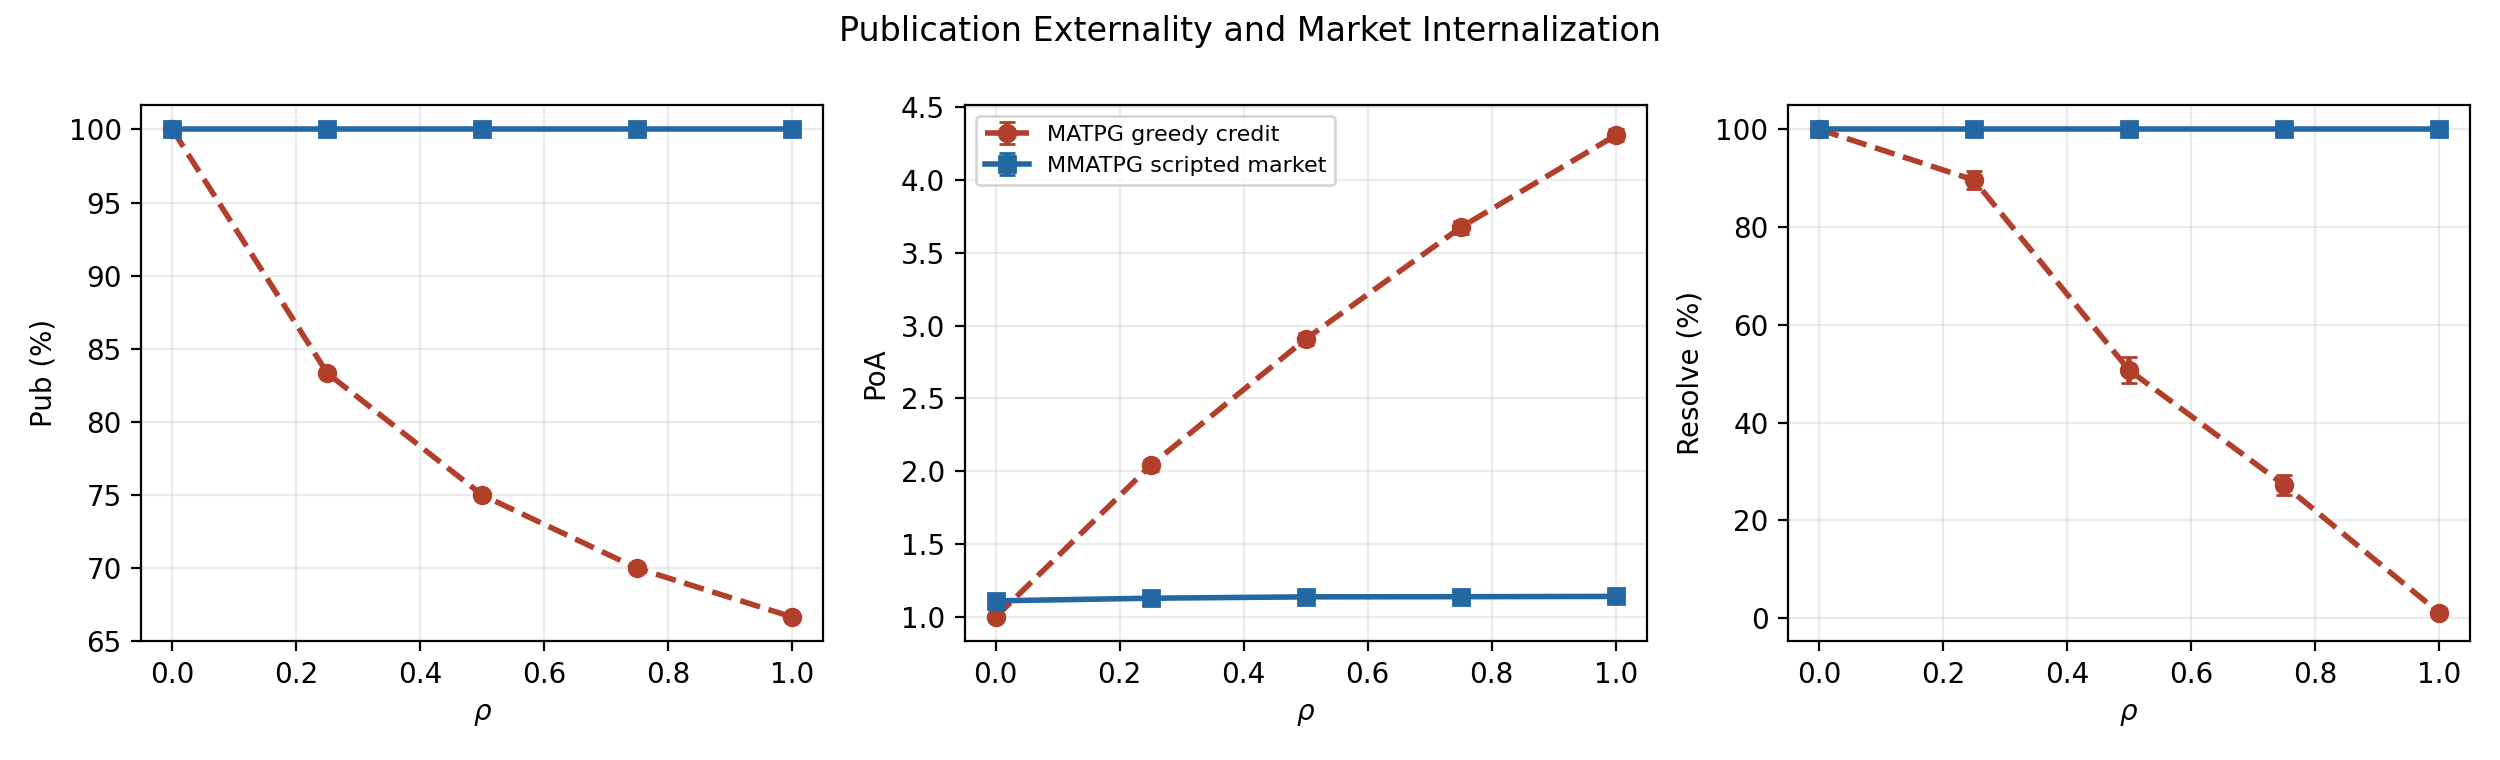
\includegraphics[width=0.9\textwidth,height=0.72\textheight,keepaspectratio]{figure_5_1_externality_market.png}

\small
Credit rewards collapse under cross-agent dependencies; market mediation keeps publication and resolution high.
\end{frame}

\begin{frame}{Experiment 2: Reading the Three Panels}
\small
\begin{itemize}
  \item \textbf{Left:} As cross-agent dependency density $\rho$ rises, greedy credit agents stop publishing byproducts. The market keeps publication near $100\%$ because settlement requires public resolution.
  \item \textbf{Middle:} No-market PoA grows sharply with dependency density; the market keeps PoA below roughly $1.25$ in this sweep.
  \item \textbf{Right:} The no-market game fails to resolve targets at high $\rho$ because dependency chains do not become public.
  \item The market result is not just a reward-shaping effect: it changes the strategic payoff of publication.
\end{itemize}
\end{frame}

\begin{frame}{Experiment 2b: Market Friction}
\centering
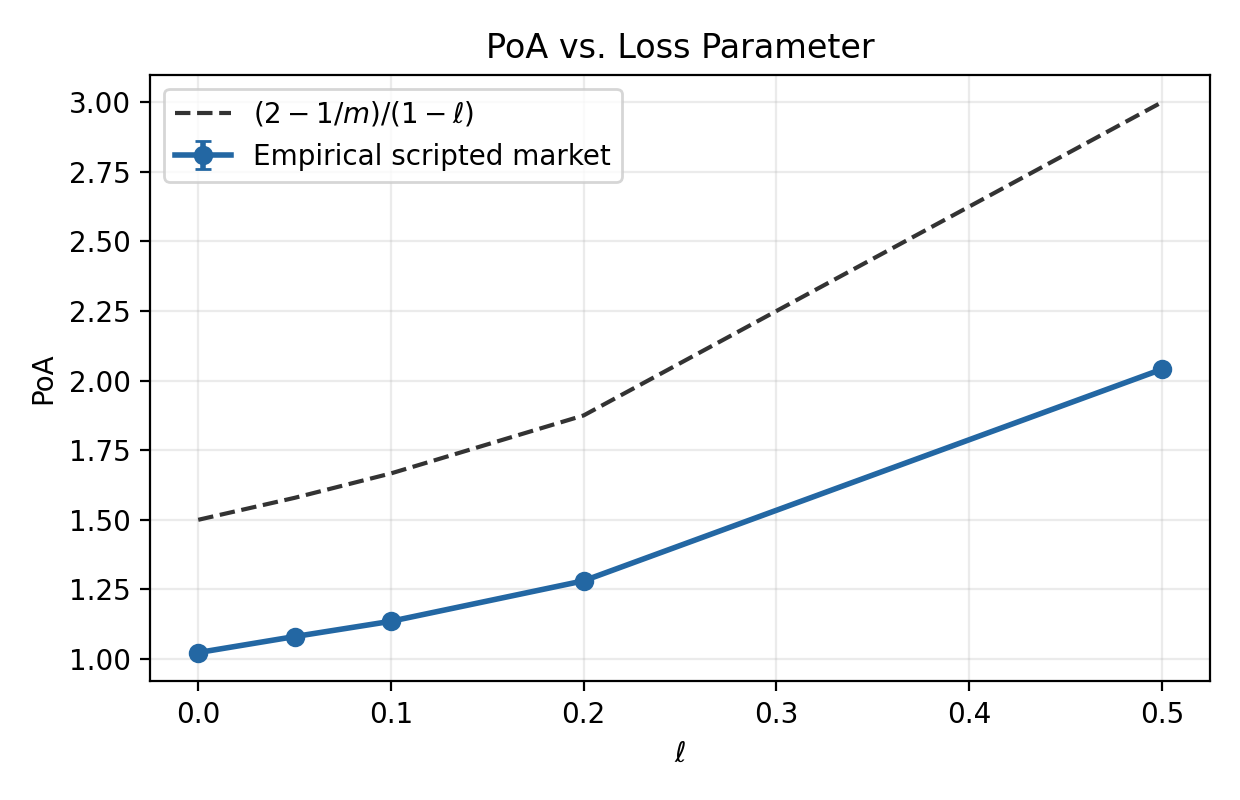
\includegraphics[width=0.82\textwidth,height=0.7\textheight,keepaspectratio]{figure_5_2_loss_poa.png}

\small
Empirical PoA tracks below the theoretical $(2-1/m)/(1-\ell)$ bound.
\end{frame}

\begin{frame}{Experiment 2b: Role of $\ell$}
\small
\begin{itemize}
  \item At $\ell=0$, a long contract is a pure bounty: no downside for the prover.
  \item Increasing $\ell$ makes long positions riskier and shrinks the prover's margin.
  \item The theorem predicts a multiplicative friction factor:
  \[
  \frac{1}{1-\ell}.
  \]
  \item The empirical curve stays below the dashed theoretical bound across the sweep.
\end{itemize}
\end{frame}

\begin{frame}{Experiment 3: Training Dynamics}
\centering
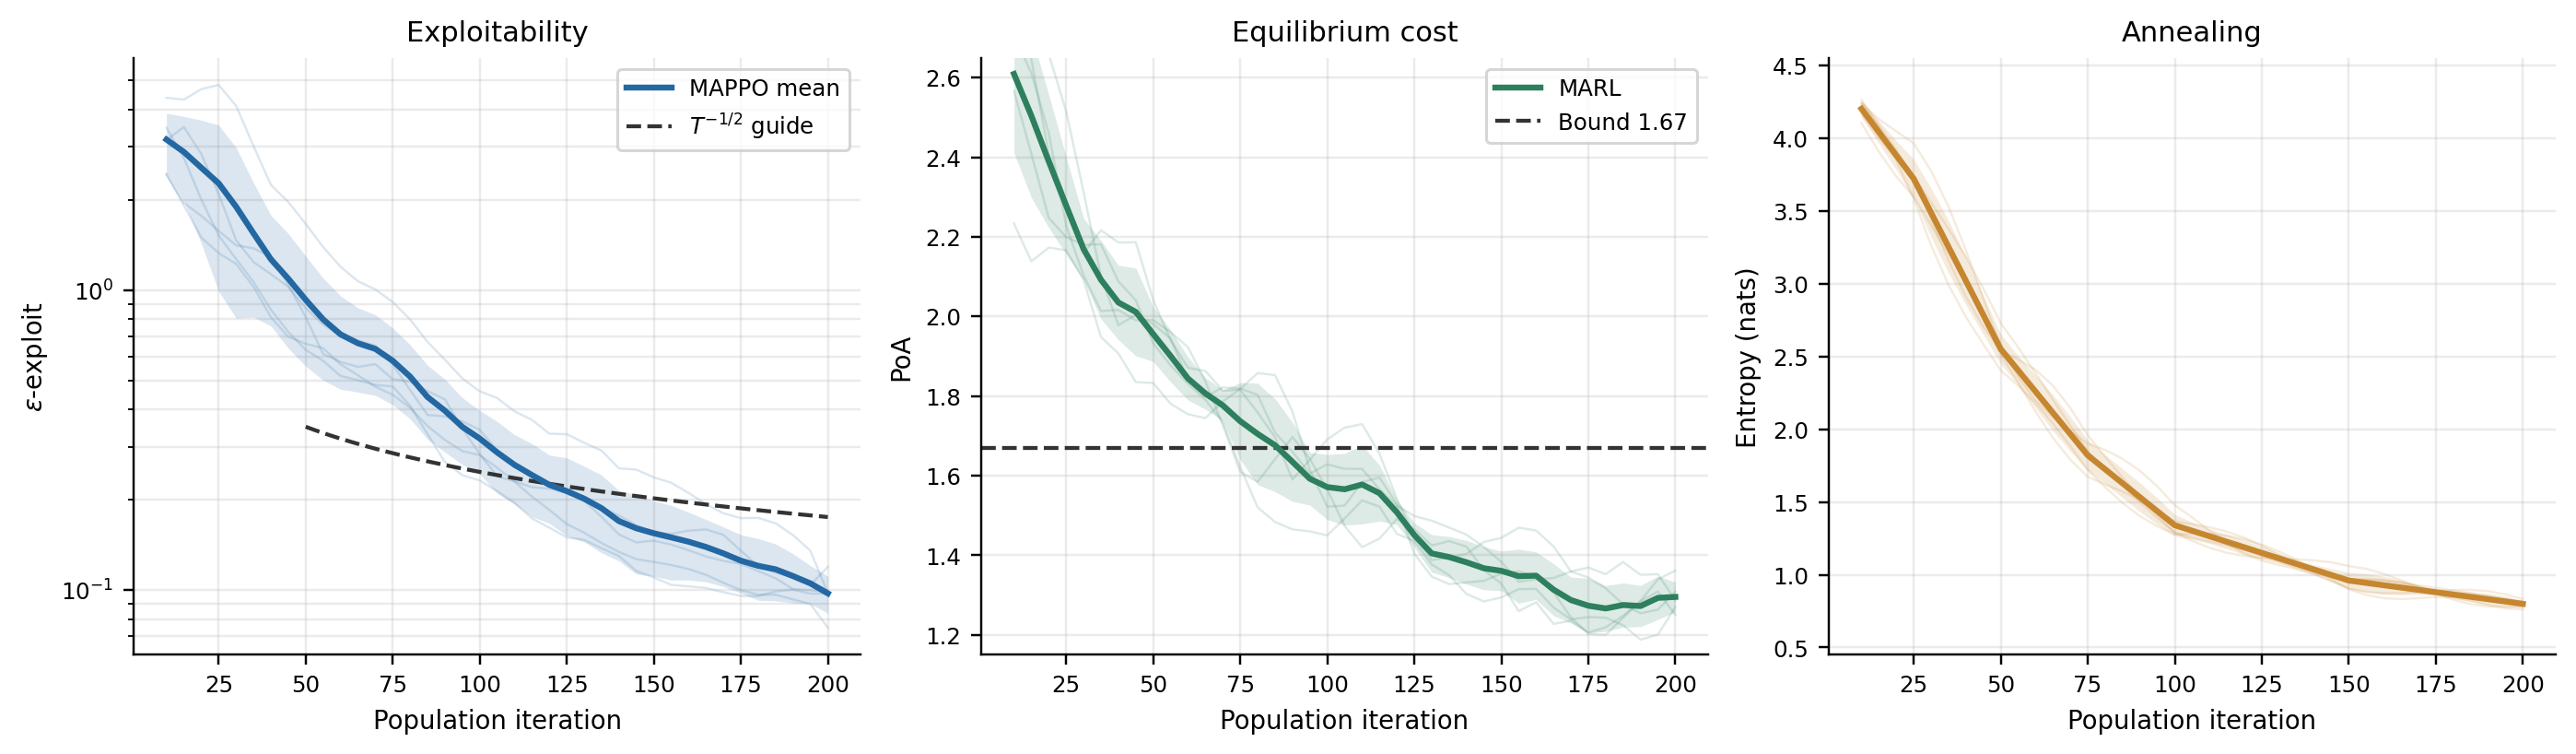
\includegraphics[width=\textwidth,height=0.72\textheight,keepaspectratio]{figure_5_3_training_dynamics.png}

\small
Exploitability follows the expected $O(1/\sqrt{T})$ trend while PoA stabilizes below the bound.
\end{frame}

\begin{frame}{Experiment 3: What Converges?}
\small
\begin{itemize}
  \item \textbf{Exploitability:} unilateral fine-tuning gains shrink, matching the approximate CCE story.
  \item \textbf{PoA:} learned play approaches a stable efficiency level below the $1.67$ theoretical bound.
  \item \textbf{Entropy:} annealing avoids premature collapse early, then sharpens decisions late.
  \item The training signal is financial balance change, but the emergent behavior improves the social makespan metric.
\end{itemize}
\end{frame}

\begin{frame}{Experiment 3: Learned Behavior}
\centering
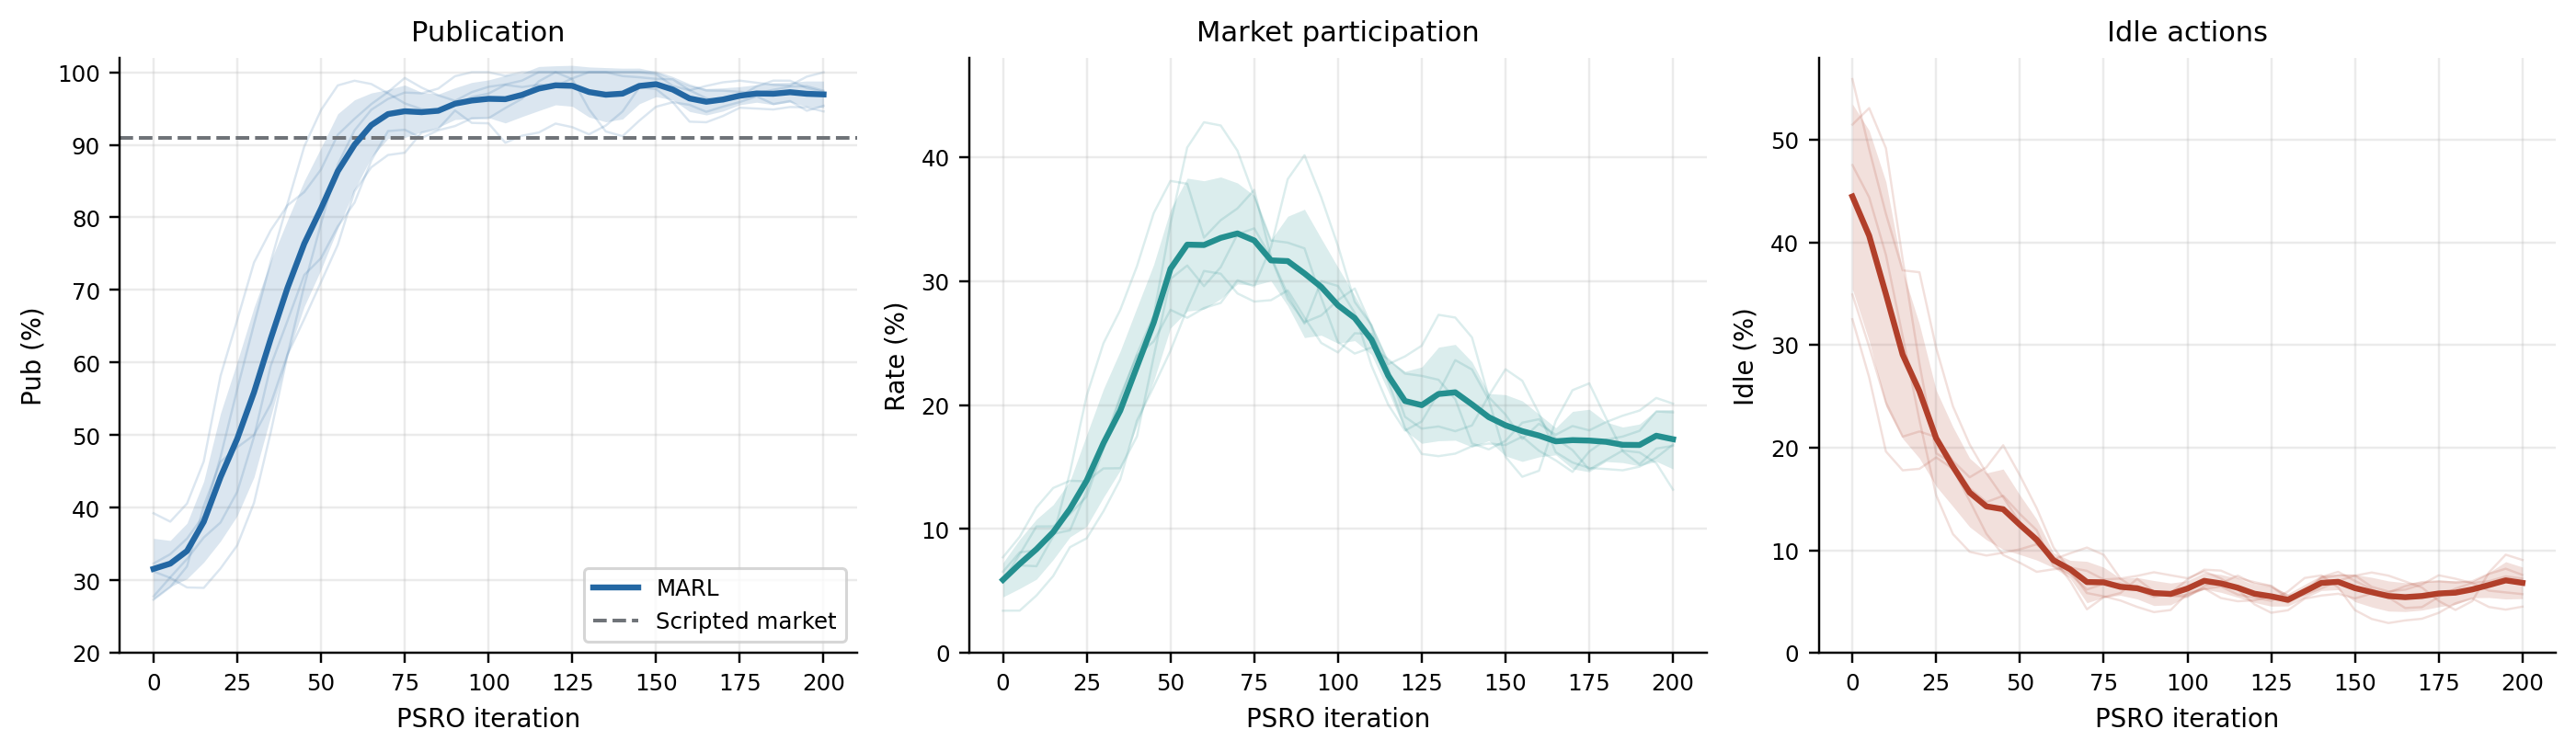
\includegraphics[width=\textwidth,height=0.72\textheight,keepaspectratio]{figure_5_4_rollout_behavior.png}

\small
Publication rises, market participation becomes selective, and idle rate falls over training.
\end{frame}

\begin{frame}{Experiment 3: Population and Best Responses}
\begin{columns}[T,onlytextwidth]
\column{0.5\textwidth}
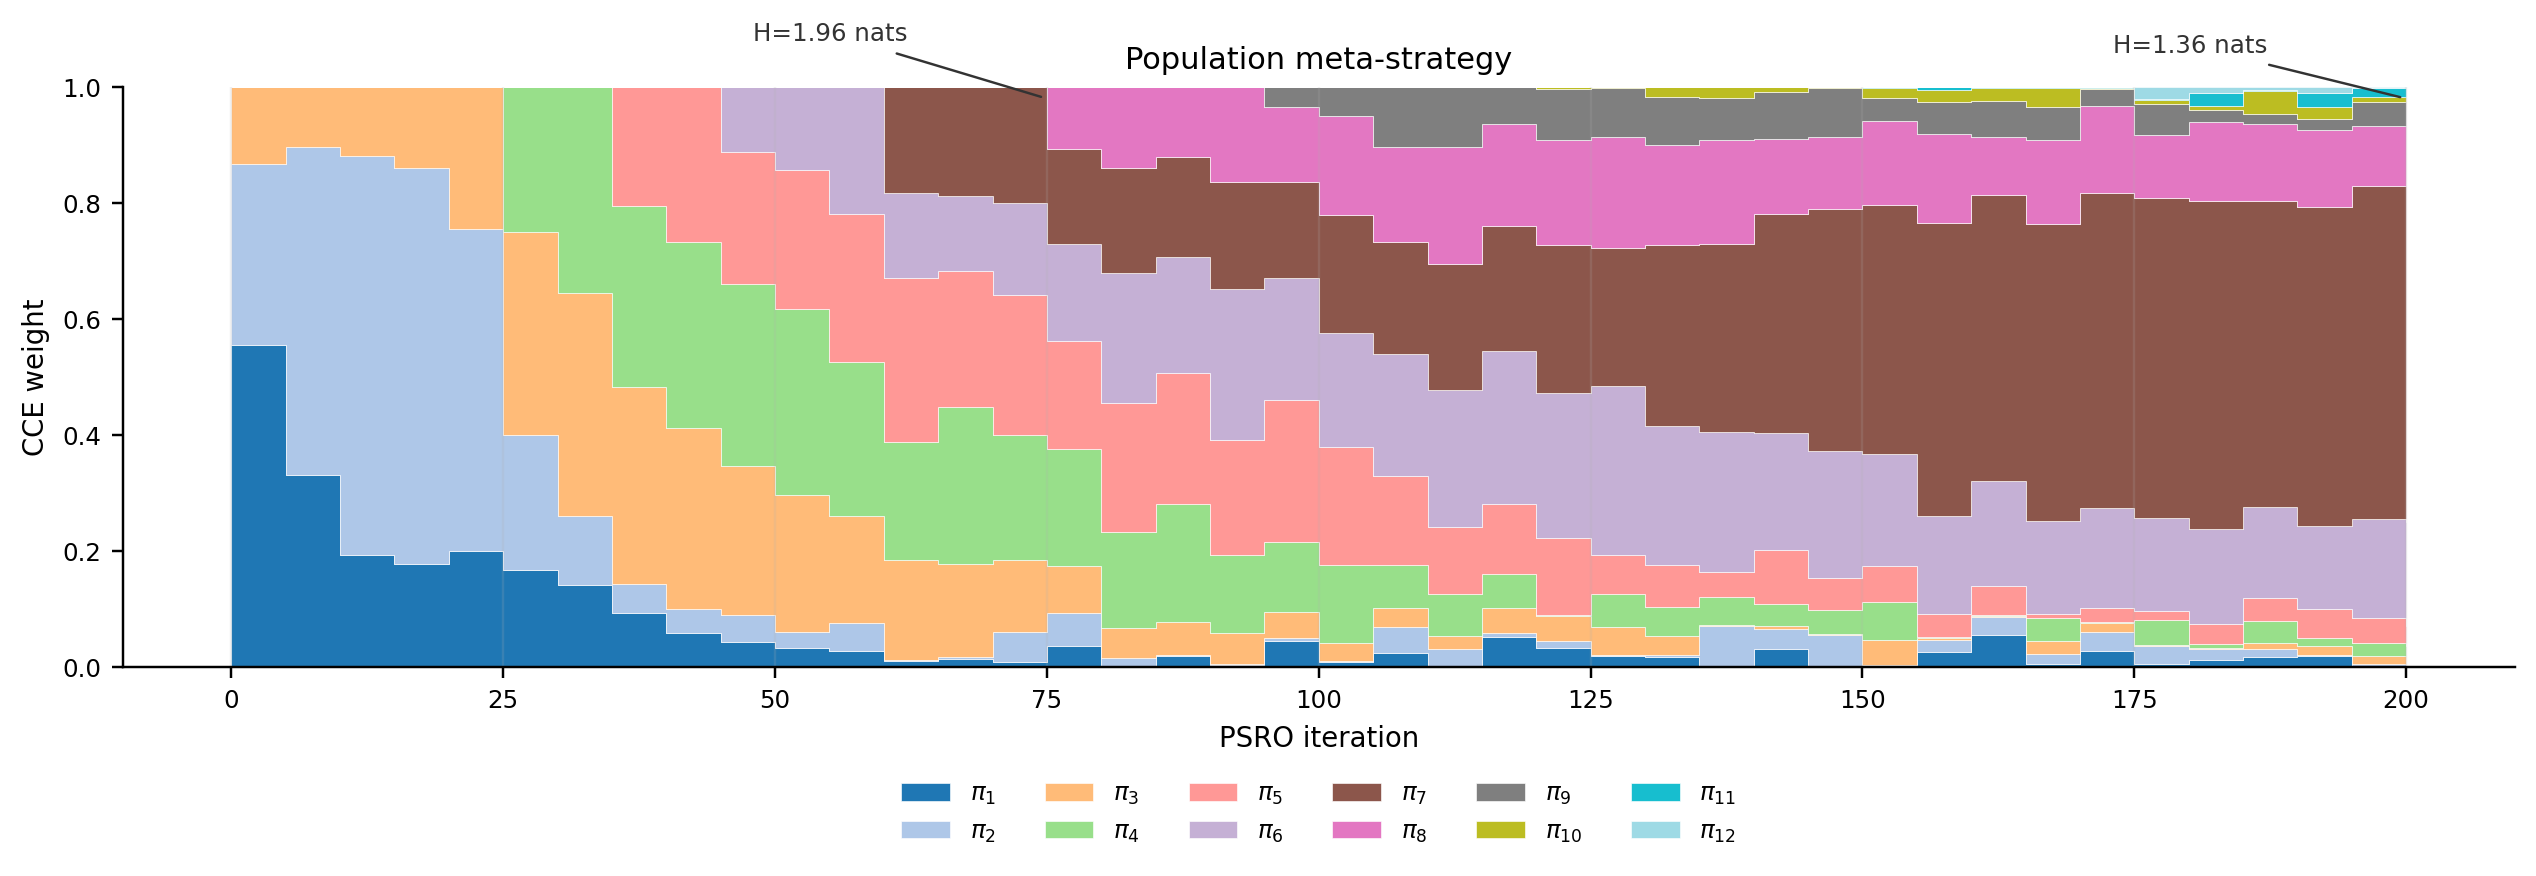
\includegraphics[width=\textwidth,height=0.61\textheight,keepaspectratio]{figure_5_5_population_metastrategy.png}
\column{0.5\textwidth}
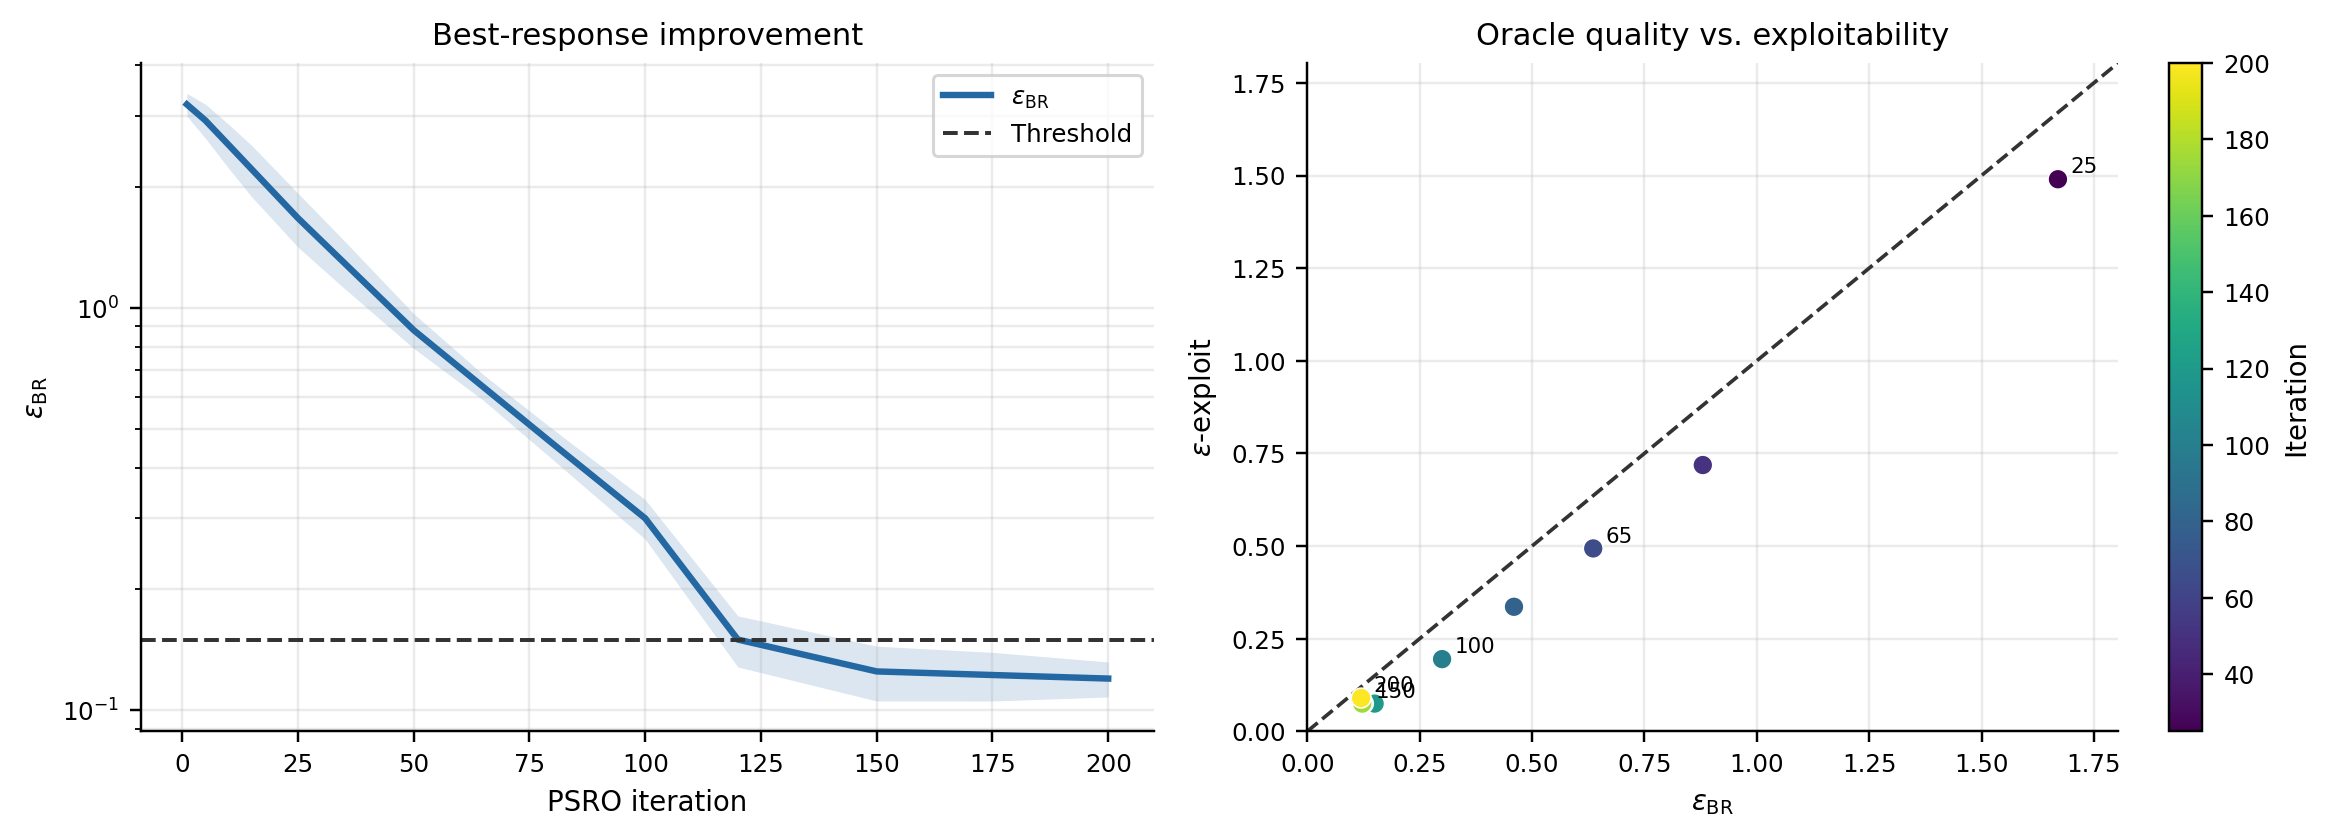
\includegraphics[width=\textwidth,height=0.61\textheight,keepaspectratio]{figure_5_6_epsbr.png}
\end{columns}

\small
Policies diversify during the middle phase, then concentrate on robust generalists as best-response gains shrink.
\end{frame}

\begin{frame}{Policy Comparison at Convergence}
\scriptsize
\centering
\resizebox{0.9\textwidth}{!}{%
\begin{tabular}{l|cccc}
\toprule
\textbf{Policy} & $\SC$ & $\PoA$ & $\varepsilon$-exploit & Resolve\% \\
\midrule
OPT (centralized)       & $27.30 \pm 1.98$ & $1.00$           & ---             & $100.0\%$ \\
Centralized RLS         & $27.98 \pm 2.18$ & $1.02 \pm 0.02$  & ---             & $100.0\%$ \\
\midrule
Greedy credit (no mkt.) & $79.11 \pm 5.38$ & $2.91 \pm 0.22$  & ---             & $50.8\%$  \\
Scripted market         & $39.47 \pm 3.21$ & $1.45 \pm 0.14$  & $0.82 \pm 0.11$ & $91.3\%$  \\
\textbf{MARL}           & $35.12 \pm 2.84$ & $1.29 \pm 0.11$  & $0.09 \pm 0.03$ & $96.7\%$  \\
\bottomrule
\end{tabular}}

\vspace{0.8em}
\small
MARL improves substantially over both no-market greedy play and a scripted market, while remaining below the theoretical PoA bound of $1.67$.
\end{frame}

\begin{frame}{Policy Comparison: Interpretation}
\small
\begin{itemize}
  \item Centralized RLS is nearly optimal on these instances: $\PoA=1.02$.
  \item Greedy credit is bad on both efficiency and completion: $\PoA=2.91$, Resolve $=50.8\%$.
  \item Scripted market fixes much of the incentive problem but remains exploitable: $\varepsilon$-exploit $=0.82$.
  \item MARL improves both coordination and equilibrium quality: $\PoA=1.29$, Resolve $=96.7\%$, exploitability $=0.09$.
\end{itemize}
\end{frame}

\begin{frame}{Ablation Summary}
\scriptsize
\centering
\resizebox{0.86\textwidth}{!}{%
\begin{tabular}{l|cccc}
\toprule
\textbf{Variant} & $\PoA$ & $\varepsilon$-exploit & Pub\% & Steps to $\varepsilon<0.15$ \\
\midrule
No market (credit + MAPPO) & $2.67 \pm 0.31$ & $2.41 \pm 0.28$ & $31.2\%$ & $>200$ \\
No population & --- & --- & --- & --- \\
No curriculum & --- & --- & --- & --- \\
No shaping & --- & --- & --- & --- \\
\textbf{Full framework} & $1.32 \pm 0.12$ & $0.11 \pm 0.04$ & $95.9\%$ & $71 \pm 11$ \\
\bottomrule
\end{tabular}}

\vspace{1em}
\small
The completed ablation already makes the largest point: learning cannot compensate for absent incentive alignment.
\end{frame}

\begin{frame}{Scaling With Task Graph Size}
\scriptsize
\centering
\resizebox{0.78\textwidth}{!}{%
\begin{tabular}{l|cccc}
\toprule
$n$ & $\PoA$ (MARL) & $\varepsilon$-exploit & Resolve\% & Wall-clock (hrs) \\
\midrule
$4$  & $1.19 \pm 0.08$ & $0.06 \pm 0.02$ & $98.4\%$ & $0.6 \pm 0.1$ \\
$8$  & $1.29 \pm 0.11$ & $0.09 \pm 0.03$ & $96.7\%$ & $1.4 \pm 0.2$ \\
$16$ & $1.41 \pm 0.14$ & $0.14 \pm 0.05$ & $93.1\%$ & $3.8 \pm 0.4$ \\
\bottomrule
\end{tabular}}

\vspace{1em}
\small
The theoretical bound is independent of $n$; empirical PoA rises mildly but remains below $1.67$.
\end{frame}

\begin{frame}{Scaling With Agent Count}
\begin{columns}[T,onlytextwidth]
\column{0.48\textwidth}
\scriptsize
\resizebox{\textwidth}{!}{%
\begin{tabular}{l|ccc}
\toprule
$m$ & $\SC$ & $\PoA$ & Bound \\
\midrule
$2$ & $35.12$ & $1.29$ & $1.67$ \\
$4$ & $24.81$ & $1.48$ & $1.94$ \\
$8$ & $19.34$ & $1.61$ & $2.08$ \\
\bottomrule
\end{tabular}}

\vspace{1em}
\small
More agents reduce absolute makespan but increase coordination surface.
\column{0.5\textwidth}
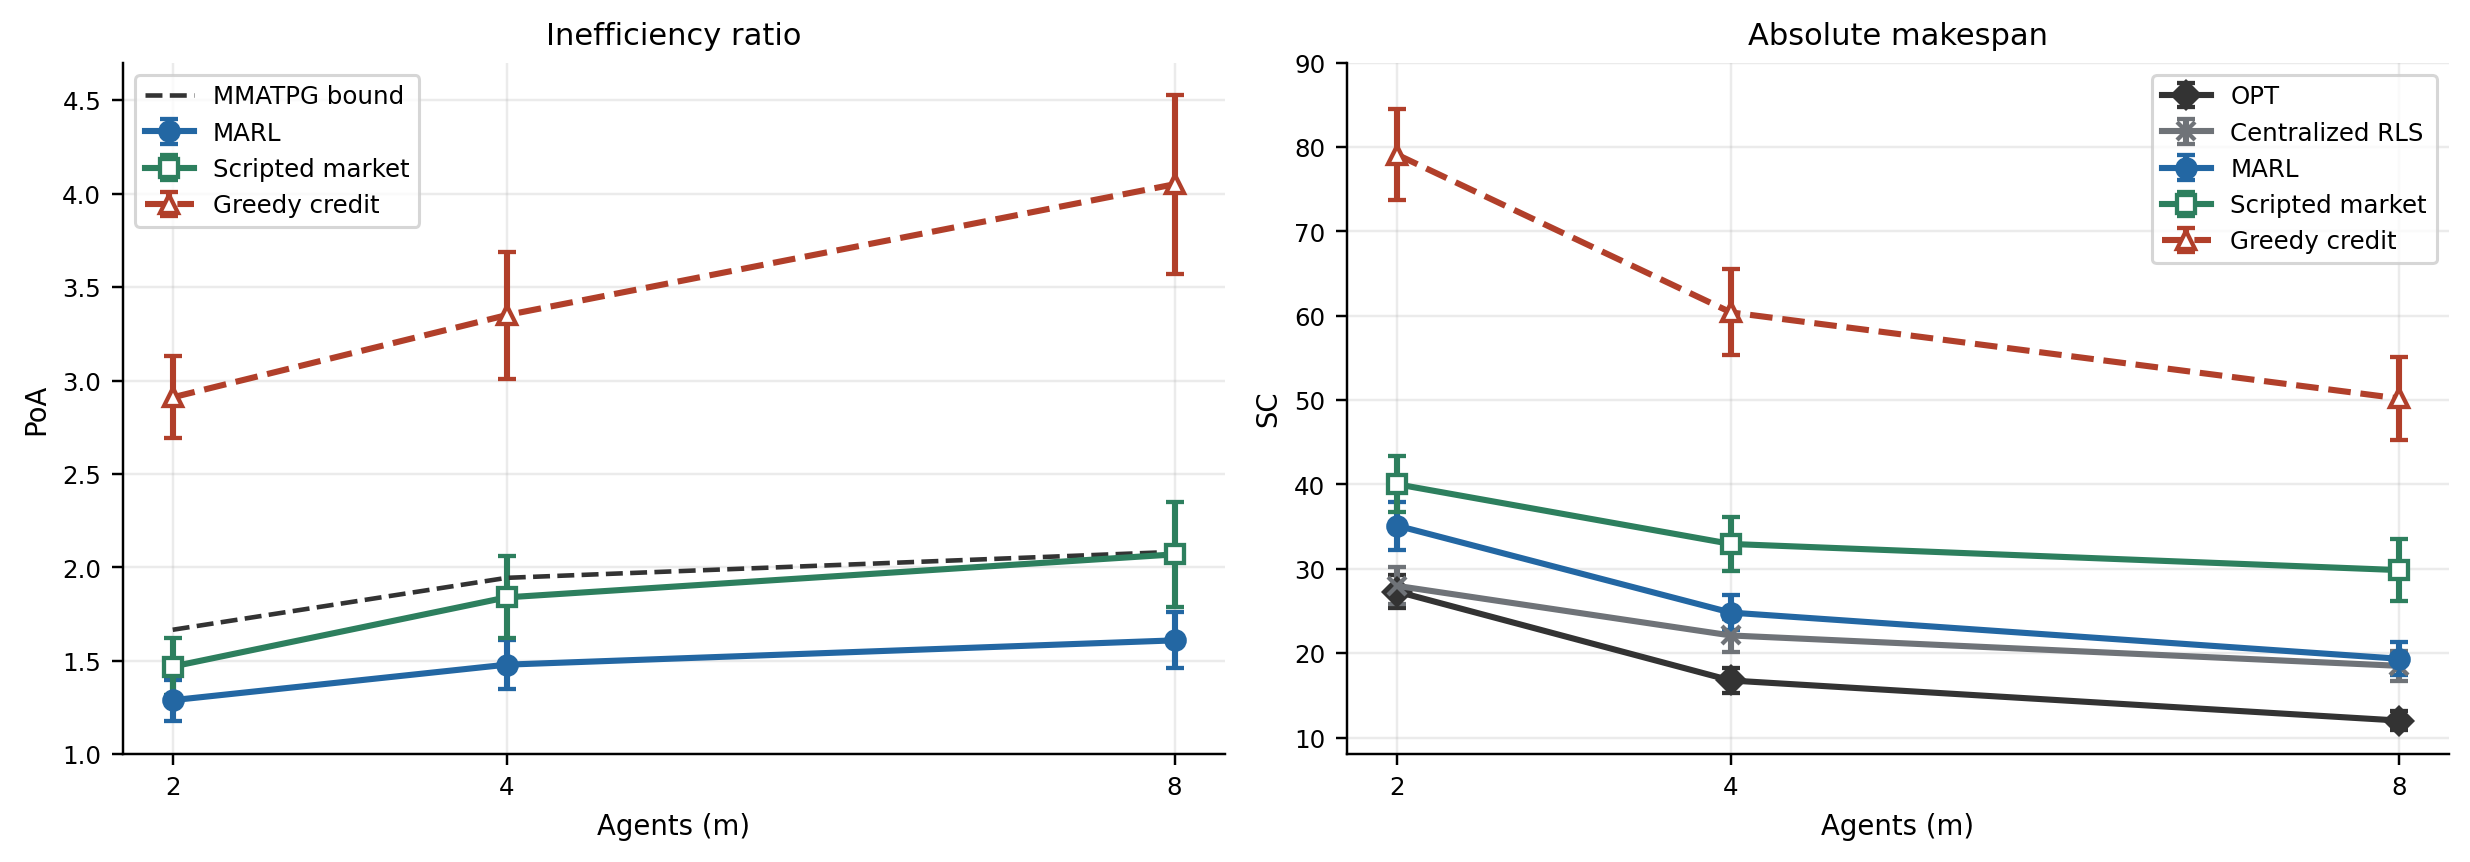
\includegraphics[width=\textwidth,height=0.58\textheight,keepaspectratio]{figure_5_7_scaling_agents.png}
\end{columns}
\end{frame}

\begin{frame}{Scaling: Main Takeaways}
\small
\begin{itemize}
  \item Larger task graphs increase exploitability and training time, but do not break the PoA story over the tested range.
  \item More agents reduce absolute makespan substantially: $35.12\to 19.34$ from $m=2$ to $m=8$.
  \item PoA rises with $m$ because coordination becomes harder, but remains below the market bound.
  \item This is the expected tradeoff: decentralization penalty grows, but parallel speedup still dominates in absolute completion time.
\end{itemize}
\end{frame}

\section{Lean Application}

\begin{frame}{Why Lean Changes the Stakes}
\small
\begin{itemize}
  \item Lean's kernel provides machine-checkable correctness.
  \item Mathlib supplies a large shared infrastructure.
  \item Formalization projects induce declaration-level dependency DAGs.
  \item Agentic LLM provers can work at project scope, but coordination is weak.
\end{itemize}

\begin{block}{Reframing}
Proof search remains local. The thesis targets the global allocation layer: which agents should try which obligations, when, and with what incentives to share intermediate results.
\end{block}
\end{frame}

\begin{frame}[plain,shrink=27]{Agora Platform}

\begin{figure}[p]
\centering
\resizebox{0.98\textwidth}{!}{%
\begin{circuitikz}
\tikzstyle{every node}=[font=\fontsize{14.2pt}{18.5pt}\selectfont]
\draw [ fill={rgb,255:red,234; green,255; blue,233}, fill opacity=1, rounded corners = 14.4] (16.25,9.875) rectangle (27.5,4.25);
\draw [ fill={rgb,255:red,255; green,236; blue,219}, fill opacity=1, rounded corners = 14.4] (16.25,16.75) rectangle (27.5,11);
\draw [ fill={rgb,255:red,255; green,255; blue,255}, fill opacity=1] (18,15.25) rectangle (20,12.5);
\draw [ fill={rgb,255:red,255; green,236; blue,236}, fill opacity=1, rounded corners = 14.4] (3.75,16.75) rectangle (10,13);
\draw [ fill={rgb,255:red,255; green,236; blue,236}, fill opacity=1, rounded corners = 14.4] (3.75,12.25) rectangle (10,8.5);
\draw [ fill={rgb,255:red,254; green,255; blue,235}, fill opacity=1, rounded corners = 14.4] (12.5,17.375) rectangle (13.75,3.625);
\draw [ fill={rgb,255:red,220; green,241; blue,255}, fill opacity=1, rounded corners = 14.4] (12.5,23) rectangle (27.5,19.25);
\node[anchor=center, align=center, inner xsep=0.080cm, inner ysep=0.085cm, rounded corners=0.020cm] at (20,21.125) {\fontsize{14.2pt}{18.5pt}\selectfont Git Repo};
\draw [ fill={rgb,255:red,246; green,228; blue,255}, fill opacity=1, rounded corners = 14.4] (30,18) rectangle (34.375,14.25);
\node[anchor=center, align=center, inner xsep=0.080cm, inner ysep=0.085cm, rounded corners=0.020cm] at (32.1875,16.125) {\fontsize{14.2pt}{18.5pt}\selectfont VerifiedAgora};
\draw [ fill={rgb,255:red,255; green,255; blue,255}, fill opacity=1] (5.5,14.875) circle (1.625cm) node[ inner xsep=0.080cm, inner ysep=0.085cm, rounded corners=0.020cm] {\fontsize{14.2pt}{18.5pt}\selectfont LLM} ;
\draw [ fill={rgb,255:red,255; green,255; blue,255}, fill opacity=1] (5.5,10.375) circle (1.625cm) node[ inner xsep=0.080cm, inner ysep=0.085cm, rounded corners=0.020cm] {\fontsize{14.2pt}{18.5pt}\selectfont LLM} ;
\draw [ fill={rgb,255:red,255; green,255; blue,255}, fill opacity=1] (23.25,15) rectangle (26,14.25);
\node[anchor=center, align=center, inner xsep=0.080cm, inner ysep=0.085cm, rounded corners=0.020cm] at (24.625,14.625) {\fontsize{10.2pt}{13.3pt}\selectfont @[target]};
\draw [ fill={rgb,255:red,255; green,255; blue,255}, fill opacity=1] (23.25,13.875) rectangle (26,13.125);
\node[anchor=center, align=center, inner xsep=0.080cm, inner ysep=0.085cm, rounded corners=0.020cm] at (24.625,13.5) {\fontsize{10.2pt}{13.3pt}\selectfont @[target]};
\draw [ fill={rgb,255:red,255; green,255; blue,255}, fill opacity=1] (23.25,12.75) rectangle (26,12);
\node[anchor=center, align=center, inner xsep=0.080cm, inner ysep=0.085cm, rounded corners=0.020cm] at (24.625,12.375) {\fontsize{10.2pt}{13.3pt}\selectfont @[target]};
\draw [ fill={rgb,255:red,255; green,236; blue,236}, fill opacity=1, rounded corners = 14.4] (3.75,8) rectangle (10,4.25);
\draw [ fill={rgb,255:red,255; green,255; blue,255}, fill opacity=1] (5.5,6.125) circle (1.625cm) node[ inner xsep=0.080cm, inner ysep=0.085cm, rounded corners=0.020cm] {\fontsize{14.2pt}{18.5pt}\selectfont LLM} ;
\draw [ fill={rgb,255:red,255; green,255; blue,255}, fill opacity=1] (17.5,9) rectangle (21.75,7.875);
\node[anchor=center, align=center, inner xsep=0.080cm, inner ysep=0.085cm, rounded corners=0.020cm] at (19.625,8.4375) {\fontsize{10.2pt}{13.3pt}\selectfont Portfolio};
\draw [ fill={rgb,255:red,255; green,255; blue,255}, fill opacity=1] (17.5,7.5) rectangle (21.75,6.375);
\node[anchor=center, align=center, inner xsep=0.080cm, inner ysep=0.085cm, rounded corners=0.020cm] at (19.625,6.9375) {\fontsize{10.2pt}{13.3pt}\selectfont Portfolio};
\draw [ fill={rgb,255:red,255; green,255; blue,255}, fill opacity=1] (17.5,6) rectangle (21.75,4.875);
\node[anchor=center, align=center, inner xsep=0.080cm, inner ysep=0.085cm, rounded corners=0.020cm] at (19.625,5.4375) {\fontsize{10.2pt}{13.3pt}\selectfont Portfolio};
\draw [ fill={rgb,255:red,255; green,255; blue,255}, fill opacity=1] (17.75,15) rectangle (19.75,12.25);
\draw [ fill={rgb,255:red,255; green,255; blue,255}, fill opacity=1] (17.5,14.75) rectangle (19.5,12);
\node[anchor=center, align=center, inner xsep=0.080cm, inner ysep=0.085cm, rounded corners=0.020cm] at (18.5,13.375) {\fontsize{14.2pt}{18.5pt}\selectfont .lean};
\draw [ fill={rgb,255:red,255; green,255; blue,255}, fill opacity=1] (24.25,8.625) rectangle (26.25,5.875);
\draw [ fill={rgb,255:red,255; green,255; blue,255}, fill opacity=1] (24,8.375) rectangle (26,5.625);
\draw [ fill={rgb,255:red,255; green,255; blue,255}, fill opacity=1] (23.75,8.125) rectangle (25.75,5.375);
\node[anchor=center, align=center, font=\fontsize{11.9pt}{15.5pt}\selectfont, inner xsep=0.080cm, inner ysep=0.085cm, rounded corners=0.020cm] at (24.75,6.75) {Contract \\ Book};
\draw [ dashed] (7.75,16.375) rectangle (9.5,13.375);
\node[anchor=center, align=center, font=\fontsize{10.2pt}{13.3pt}\selectfont, inner xsep=0.080cm, inner ysep=0.085cm, rounded corners=0.020cm] at (8.625,14.875) {Local \\ Container};
\draw [ dashed] (7.75,11.875) rectangle (9.5,8.875);
\node[anchor=center, align=center, font=\fontsize{10.2pt}{13.3pt}\selectfont, inner xsep=0.080cm, inner ysep=0.085cm, rounded corners=0.020cm] at (8.625,10.375) {Local \\ Container};
\draw [ dashed] (7.75,7.625) rectangle (9.5,4.625);
\node[anchor=center, align=center, font=\fontsize{10.2pt}{13.3pt}\selectfont, inner xsep=0.080cm, inner ysep=0.085cm, rounded corners=0.020cm] at (8.625,6.125) {Local \\ Container};
\draw [{Stealth[scale=1.5]}-{Stealth[scale=1.5]}, ] (10,14.75) -- (12.375,14.75);
\draw [{Stealth[scale=1.5]}-{Stealth[scale=1.5]}, ] (10,10.25) -- (12.375,10.25);
\draw [{Stealth[scale=1.5]}-{Stealth[scale=1.5]}, ] (10,6) -- (12.5,6);
\draw [short] (32.5,18) -- (32.5,21.625);
\draw [-{Stealth[scale=1.5]}, ] (32.5,21.625) -- (27.5,21.625);
\draw [short] (12.5,21.125) -- (1.25,21.125);
\draw [short] (1.25,21.125) -- (1.25,6);
\draw [-{Stealth[scale=1.5]}, ] (1.25,6) -- (3.625,6);
\draw [-{Stealth[scale=1.5]}, ] (1.25,10.5) -- (3.625,10.5);
\draw [-{Stealth[scale=1.5]}, ] (1.25,15) -- (3.75,15);
\draw [short] (27.5,13) -- (32.5,13);
\draw [-{Stealth[scale=1.5]}, ] (32.5,13) -- (32.5,14.25);
\draw [-{Stealth[scale=1.5]}, ] (30,15.5) -- (27.5,15.5);
\draw [{Stealth[scale=1.5]}-{Stealth[scale=1.5]}, ] (23.25,14.625) -- (20.125,14.625);
\draw [{Stealth[scale=1.5]}-{Stealth[scale=1.5]}, ] (23.25,13.5) -- (20.125,13.5);
\draw [{Stealth[scale=1.5]}-{Stealth[scale=1.5]}, ] (23.25,12.375) -- (20.125,12.375);
\draw [{Stealth[scale=1.5]}-{Stealth[scale=1.5]}, ] (21.75,8.375) -- (23.625,8.375);
\draw [{Stealth[scale=1.5]}-{Stealth[scale=1.5]}, ] (21.75,6.875) -- (23.625,6.875);
\draw [{Stealth[scale=1.5]}-{Stealth[scale=1.5]}, ] (21.75,5.5) -- (23.625,5.5);
\draw [-{Stealth[scale=1.5]}, ] (25,11) -- (25,9.875);
\draw [-{Stealth[scale=1.5]}, ] (13.75,14.75) -- (16.25,14.75);
\draw [-{Stealth[scale=1.5]}, ] (16.25,13) -- (13.75,13);
\draw [-{Stealth[scale=1.5]}, ] (13.75,6.25) -- (16.25,6.25);
\draw [-{Stealth[scale=1.5]}, ] (16.25,7.5) -- (13.75,7.5);
\node [font=\fontsize{11.9pt}{15.5pt}\selectfont, inner xsep=0.080cm, inner ysep=0.085cm, rounded corners=0.020cm] at (6.75,3.75) {Agent Orchestrator};
\node [font=\fontsize{11.9pt}{15.5pt}\selectfont, inner xsep=0.080cm, inner ysep=0.085cm, rounded corners=0.020cm] at (13.125,3.125) {Backend Interface};
\node [font=\fontsize{11.9pt}{15.5pt}\selectfont, inner xsep=0.080cm, inner ysep=0.085cm, rounded corners=0.020cm] at (22,3.75) {Market Mechanics};
\node [font=\fontsize{11.9pt}{15.5pt}\selectfont, inner xsep=0.080cm, inner ysep=0.085cm, rounded corners=0.020cm] at (22.125,17.125) {Library Mechanics};
\node [font=\fontsize{11.9pt}{15.5pt}\selectfont, inner xsep=0.080cm, inner ysep=0.085cm, rounded corners=0.020cm] at (30.125,12.625) {Request};
\node [font=\fontsize{11.9pt}{15.5pt}\selectfont, inner xsep=0.080cm, inner ysep=0.085cm, rounded corners=0.020cm] at (28.875,15.875) {Resolve};
\node [font=\fontsize{11.9pt}{15.5pt}\selectfont, inner xsep=0.080cm, inner ysep=0.085cm, rounded corners=0.020cm] at (30.25,22) {Git Push};
\node [font=\fontsize{11.9pt}{15.5pt}\selectfont, inner xsep=0.080cm, inner ysep=0.085cm, rounded corners=0.020cm] at (6.375,21.5) {Git Pull};
\node [font=\fontsize{11.9pt}{15.5pt}\selectfont, inner xsep=0.080cm, inner ysep=0.085cm, rounded corners=0.020cm] at (15,5.875) {Response};
\node [font=\fontsize{11.9pt}{15.5pt}\selectfont, inner xsep=0.080cm, inner ysep=0.085cm, rounded corners=0.020cm, align=center] at (15,8.375) {~ \\ Market \\ Request};
\node [font=\fontsize{11.9pt}{15.5pt}\selectfont, inner xsep=0.080cm, inner ysep=0.085cm, rounded corners=0.020cm] at (15,12.625) {Response};
\node [font=\fontsize{11.9pt}{15.5pt}\selectfont, inner xsep=0.080cm, inner ysep=0.085cm, rounded corners=0.020cm, align=center] at (15,15.375) {Library \\ Request};
\node [font=\fontsize{11.9pt}{15.5pt}\selectfont, inner xsep=0.080cm, inner ysep=0.085cm, rounded corners=0.020cm] at (11.25,15.125) {MCP};
\node [font=\fontsize{11.9pt}{15.5pt}\selectfont, inner xsep=0.080cm, inner ysep=0.085cm, rounded corners=0.020cm] at (11.25,10.625) {MCP};
\node [font=\fontsize{11.9pt}{15.5pt}\selectfont, inner xsep=0.080cm, inner ysep=0.085cm, rounded corners=0.020cm] at (11.25,6.25) {MCP};
\node [font=\fontsize{11.9pt}{15.5pt}\selectfont, inner xsep=0.080cm, inner ysep=0.085cm, rounded corners=0.000cm] at (21.625,13.75) {};
\node [font=\fontsize{11.9pt}{15.5pt}\selectfont, inner xsep=0.080cm, inner ysep=0.085cm, rounded corners=0.020cm] at (22.75,7.125) {Trade};
\node [font=\fontsize{11.9pt}{15.5pt}\selectfont, inner xsep=0.080cm, inner ysep=0.085cm, rounded corners=0.020cm] at (27.25,10.5) {Init/Resolution Updates};
\end{circuitikz}
}%
\caption{Agora platform architecture. Library Mechanics owns Lean validation; Market Mechanics owns financial invariants; the Backend Interface exposes MCP tools to LLM agents. The Agent Orchestrator provisions containers and seeds the market.}
\label{fig:agora-arch}
\end{figure}


\end{frame}

\begin{frame}{VerifiedAgora}
\small
\begin{itemize}
  \item Targets are Lean declarations tagged with \texttt{@[target]}.
  \item Unresolved targets may contain \texttt{sorryAx}; solved targets must be sorry-free.
  \item Non-target declarations are checked against a strict axiom policy.
  \item Submitted content is compiled, matched against target descriptors, automerged if valid, then rebuilt.
  \item Invalid contributions are rejected without breaking the shared repository.
\end{itemize}

\begin{block}{Trust boundary}
LLM agents may generate arbitrary text; only Lean and VerifiedAgora decide what becomes public mathematical state.
\end{block}
\end{frame}

\begin{frame}{Mapping Agora to MMATPG}
\small
\begin{tabular}{p{0.27\textwidth}p{0.62\textwidth}}
\toprule
\textbf{MMATPG object} & \textbf{Agora/Lean instantiation} \\
\midrule
Formula & Lean declaration of type \texttt{Prop}. \\
Library & Shared branch plus each agent's local workspace. \\
Resolution & VerifiedAgora-certified sorry-free target. \\
Dependencies & Extracted from Lean environment after proof checking. \\
Publication & Contribution accepted and committed to shared branch. \\
Market contract & Target-conditioned asset settled by target resolution. \\
Proof kernel & LLM proof attempt plus Lean binary oracle. \\
Query model & LLM estimate of success probability and duration. \\
\bottomrule
\end{tabular}
\end{frame}

\begin{frame}{Training Data for the Strategy Module}
\small
\begin{itemize}
  \item Real Lean training is too expensive for repeated MARL rollouts.
  \item Extract dependency DAG and difficulty statistics from the target repository.
  \item Generate synthetic DAGs with similar depth, clustering, degree, rarity, and utility structure.
  \item Train strategy module synthetically, deploy zero-shot into Agora prompts.
\end{itemize}

\begin{block}{Training-to-inference gap}
The synthetic kernel is stationary and Markovian; real LLM agents are not. The deployment uses soft prompt recommendations so the LLM can deviate.
\end{block}
\end{frame}

% \begin{frame}{PNT-Calibrated Synthetic Graphs}
% \centering
% \scriptsize
% \begin{tabular}{c}
% \textbf{Extracted PNT utility graph}\\
% \includegraphics[width=0.78\textwidth,height=0.25\textheight,keepaspectratio]{pnt_synth_og.pdf}
% \end{tabular}

% \vspace{0.15em}
% \begin{tabular}{cc}
% \includegraphics[width=0.46\textwidth,height=0.19\textheight,keepaspectratio]{pnt_synth_1024.pdf} &
% \includegraphics[width=0.46\textwidth,height=0.19\textheight,keepaspectratio]{pnt_synth_512.pdf}\\
% \includegraphics[width=0.46\textwidth,height=0.19\textheight,keepaspectratio]{pnt_synth_256.pdf} &
% \includegraphics[width=0.46\textwidth,height=0.19\textheight,keepaspectratio]{pnt_synth_128.pdf}
% \end{tabular}

% \vspace{0.2em}
% The generator preserves dependency geometry while allowing many fresh training episodes.
% \end{frame}

\begin{frame}{PNT-Calibrated Synthetic Graphs}
\centering
\scriptsize
\textbf{Extracted PNT utility graph}\\
\begin{minipage}[c]{0.48\textwidth}
    \centering
    
    \includegraphics[
        width=\textwidth,
        height=0.7\textheight,
        keepaspectratio
    ]{pnt_synth_og.pdf}
\end{minipage}
\hfill
\begin{minipage}[c]{0.48\textwidth}
    \centering
    \begin{tabular}{cc}
        \includegraphics[width=0.47\textwidth,height=0.35\textheight,keepaspectratio]{pnt_synth_1024.pdf} &
        \includegraphics[width=0.47\textwidth,height=0.35\textheight,keepaspectratio]{pnt_synth_512.pdf} \\
        \includegraphics[width=0.47\textwidth,height=0.35\textheight,keepaspectratio]{pnt_synth_256.pdf} &
        \includegraphics[width=0.47\textwidth,height=0.35\textheight,keepaspectratio]{pnt_synth_128.pdf}
    \end{tabular}
\end{minipage}

\vspace{0.4em}

The generator preserves dependency geometry while allowing many fresh training episodes.
\end{frame}

\begin{frame}{PNT Benchmark}
\small
\begin{columns}[T,onlytextwidth]
\column{0.45\textwidth}
\begin{block}{MiniCTX PNT}
\begin{tabular}{lr}
\toprule
Metric & Value \\
\midrule
Total declarations & 911 \\
Sorry targets & 92 \\
DAG depth & 18 \\
Avg. dependencies per target & 0.30 \\
Easy / Medium / Hard & 39 / 41 / 12 \\
\bottomrule
\end{tabular}
\end{block}
\column{0.5\textwidth}
\begin{itemize}
  \item Systems fill sorry'd targets under a fixed wall-clock budget.
  \item Agora systems use verified publication and market bounties.
  \item Strategy variant adds learned recommendations at each decision epoch.
\end{itemize}
\end{columns}
\end{frame}

\begin{frame}{Systems Under Comparison}
\small
\begin{tabular}{p{0.16\textwidth}p{0.74\textwidth}}
\toprule
\textbf{System} & \textbf{Role in evaluation} \\
\midrule
A1 & Single Claude Code agent with Lean LSP: serial proof-search baseline. \\
A2 & Claude Code Teams with 8 agents: parallelism without explicit market/strategy coordination. \\
A3 & Aristotle Agent: purpose-built SOTA agentic Lean prover. \\
A4 & OpenGauss: second SOTA black-box theorem-proving baseline. \\
B1 & Agora scaffold with 8 agents: verified publication, shared branch, and market bounties. \\
C1 & Agora + Strategy: B1 plus the MARL-trained allocation policy injected into agent prompts. \\
\bottomrule
\end{tabular}
\end{frame}

\begin{frame}{PNT Proof Completion}
\scriptsize
\centering
\resizebox{0.9\textwidth}{!}{%
\begin{tabular}{ll|cccc}
\toprule
& \textbf{System} & \textbf{Easy} & \textbf{Med.} & \textbf{Hard} & \textbf{Overall} \\
\midrule
& Claude Code (1) & 8 (21\%) & 2 (5\%) & 0 (0\%) & 10 (11\%) \\
& Claude Code Teams (8) & 15 (38\%) & 5 (12\%) & 0 (0\%) & 20 (22\%) \\
& Aristotle Agent & 35 (90\%) & 28 (68\%) & 5 (42\%) & 68 (74\%) \\
& OpenGauss & 32 (82\%) & 22 (54\%) & 3 (25\%) & 57 (62\%) \\
\midrule
& Agora Scaffold (8) & 20 (51\%) & 10 (24\%) & 1 (8\%) & 31 (34\%) \\
\midrule
& \textbf{Agora + Strategy (8)} & \textbf{28 (72\%)} & \textbf{17 (41\%)} & \textbf{3 (25\%)} & \textbf{48 (52\%)} \\
\bottomrule
\end{tabular}}

\vspace{0.8em}
\small
The strategy module improves most on medium and hard targets, where dependency-aware allocation matters.
\end{frame}

\begin{frame}{PNT Proof Completion: Walkthrough}
\small
\begin{itemize}
  \item \textbf{A1 to A2:} parallelism alone doubles completion from $11\%$ to $22\%$, but hard targets remain unsolved.
  \item \textbf{A2 to B1:} verified publication and market bounties improve completion to $34\%$ by reducing duplicate work and making shared progress immediately useful.
  \item \textbf{B1 to C1:} the learned strategy raises overall completion to $52\%$.
  \item The improvement concentrates on \textbf{Medium} and \textbf{Hard} targets, matching the thesis claim that dependency-aware allocation matters most when proof obligations interact.
  \item Purpose-built SOTA systems still lead overall; the point is that the coordination layer closes a large fraction of the gap without replacing the prover.
\end{itemize}
\end{frame}

\begin{frame}{Anytime Performance}
\centering
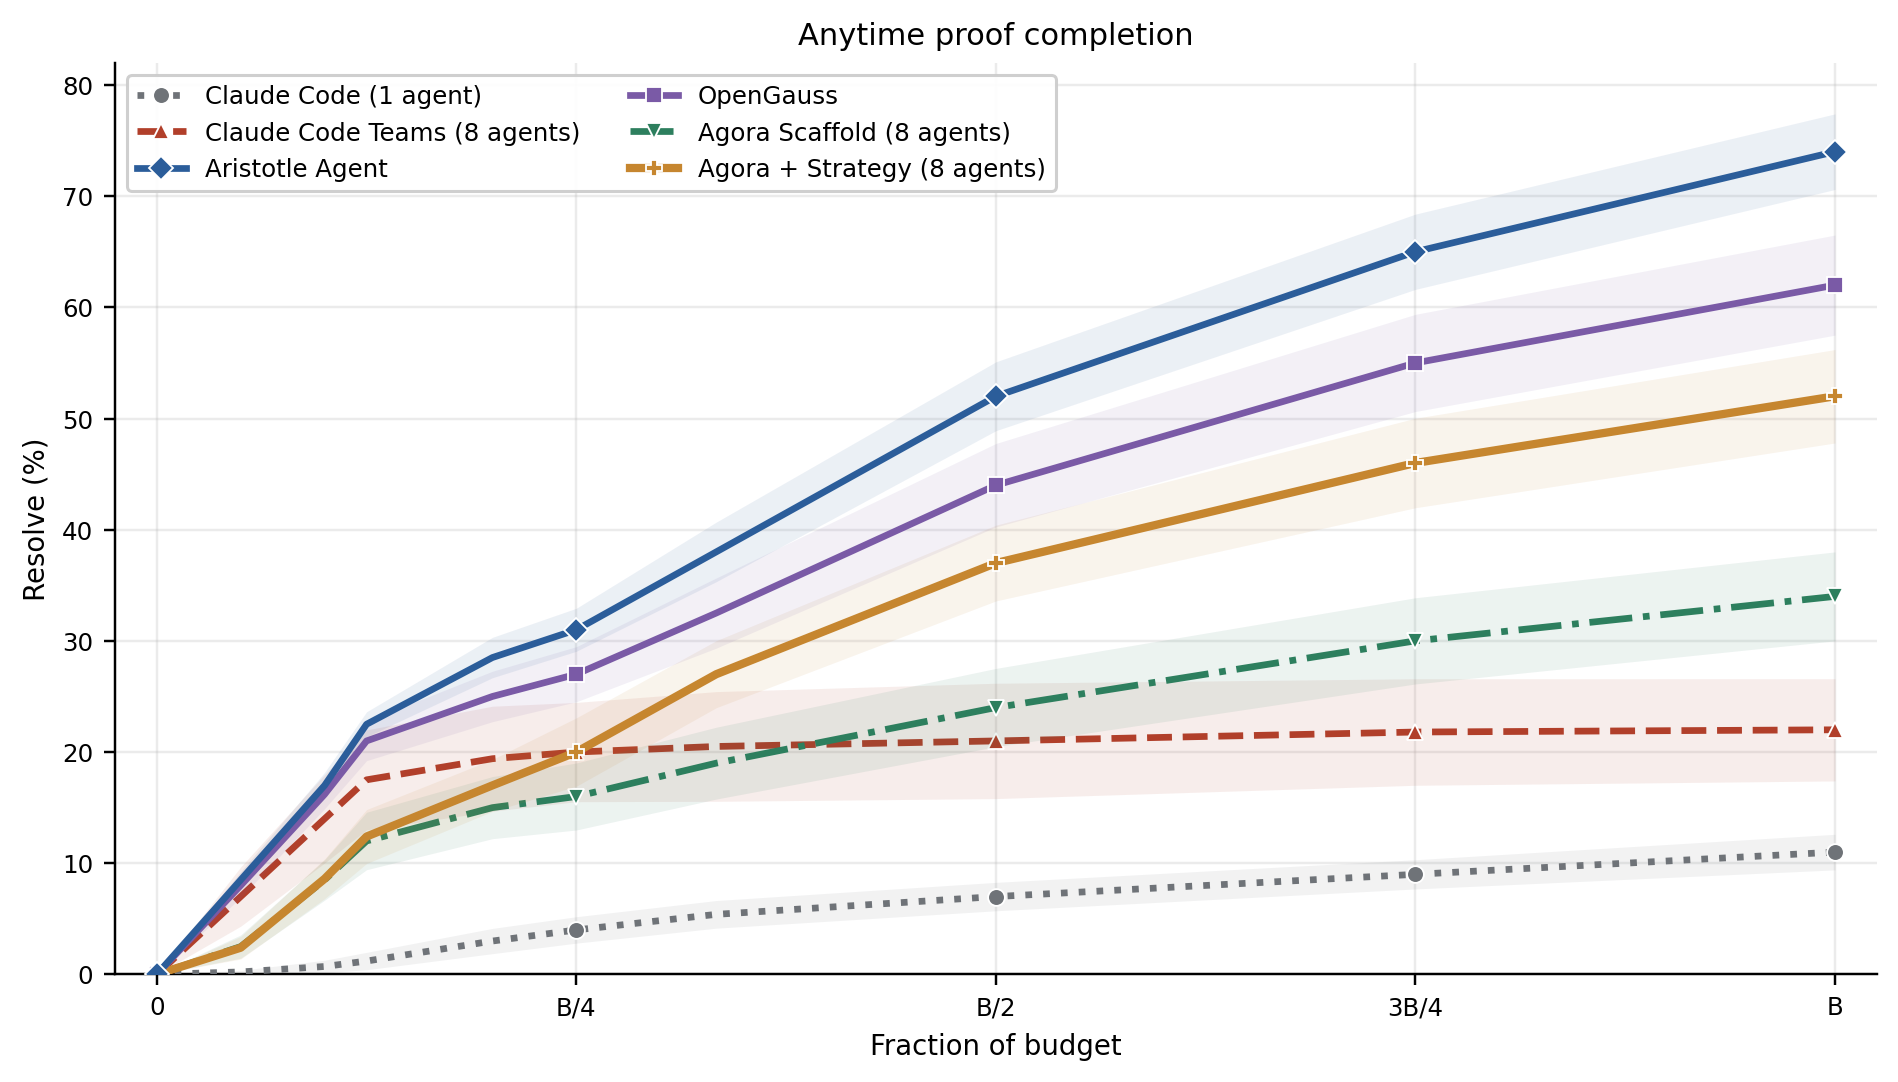
\includegraphics[width=0.9\textwidth,height=0.72\textheight,keepaspectratio]{figure_6_3_anytime_performance.png}

\small
Agora + Strategy resolves more targets earlier, not only more targets by the final budget.
\end{frame}

\begin{frame}{Coordination Metrics}
\small
\centering
\begin{tabular}{l|ccc}
\toprule
\textbf{System} & Duplication\% $\downarrow$ & DepUnlock $\uparrow$ & API calls \\
\midrule
Claude Code Teams & $36\%$ & 2 & --- \\
Agora Scaffold & $21\%$ & 5 & --- \\
\textbf{Agora + Strategy} & \textbf{$8\%$} & \textbf{9} & --- \\
\bottomrule
\end{tabular}

\vspace{1em}
\begin{itemize}
  \item The scaffold reduces duplication through shared state and markets.
  \item The learned strategy further prioritizes dependency-unlocking work.
  \item This is the empirical signature of allocation improvement.
\end{itemize}
\end{frame}

\begin{frame}{Coordination Metrics: Interpretation}
\small
\begin{itemize}
  \item \textbf{Duplication\%} measures wasted parallelism: multiple agents attempting work already solved or being solved elsewhere.
  \item \textbf{DepUnlock} counts events where one publication makes downstream targets newly feasible or easier.
  \item Claude Code Teams has high duplication because coordination is mostly implicit through files.
  \item Agora Scaffold reduces duplication through shared state and bounty signals.
  \item Agora + Strategy reduces duplication to $8\%$ and almost doubles dependency unlocks relative to the scaffold.
\end{itemize}
\end{frame}

\begin{frame}{Case Study Dependency DAG}
\small
\begin{center}
\resizebox{!}{0.58\textheight}{%
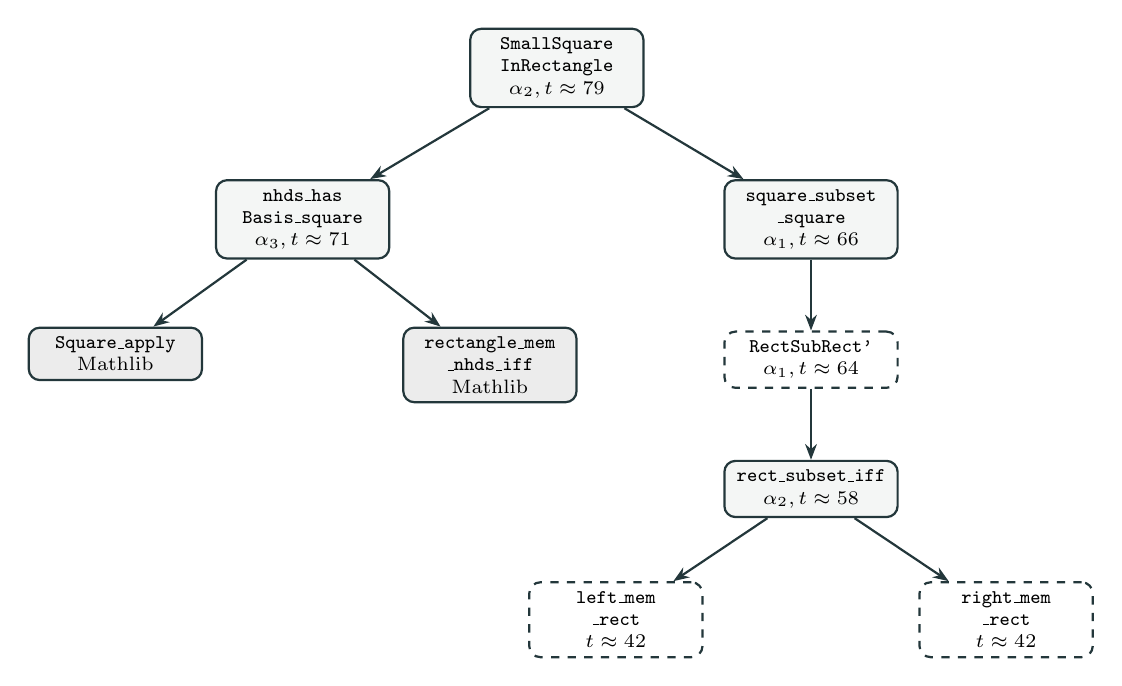
\begin{tikzpicture}[
  node/.style={draw=mDarkTeal,thick,rounded corners,fill=mLight,align=center,minimum width=2.2cm,minimum height=0.62cm,font=\scriptsize},
  conj/.style={node,dashed,fill=white},
  target/.style={node,fill=mLight},
  arr/.style={-{Stealth[length=2mm]},thick,mDarkTeal}
]
\node[target] (top) {\texttt{SmallSquare}\\\texttt{InRectangle}\\$\alpha_2,t\approx79$};
\node[target,below left=0.9cm and 1.0cm of top] (nhds) {\texttt{nhds\_has}\\\texttt{Basis\_square}\\$\alpha_3,t\approx71$};
\node[target,below right=0.9cm and 1.0cm of top] (sqsub) {\texttt{square\_subset}\\\texttt{\_square}\\$\alpha_1,t\approx66$};
\node[node,fill=gray!15,below left=0.85cm and 0.15cm of nhds] (sqapply) {\texttt{Square\_apply}\\Mathlib};
\node[node,fill=gray!15,below right=0.85cm and 0.15cm of nhds] (rectnhds) {\texttt{rectangle\_mem}\\\texttt{\_nhds\_iff}\\Mathlib};
\node[conj,below=0.9cm of sqsub] (rectsub) {\texttt{RectSubRect'}\\$\alpha_1,t\approx64$};
\node[target,below=0.9cm of rectsub] (iff) {\texttt{rect\_subset\_iff}\\$\alpha_2,t\approx58$};
\node[conj,below left=0.8cm and 0.25cm of iff] (left) {\texttt{left\_mem}\\\texttt{\_rect}\\$t\approx42$};
\node[conj,below right=0.8cm and 0.25cm of iff] (right) {\texttt{right\_mem}\\\texttt{\_rect}\\$t\approx42$};
\draw[arr] (top) -- (nhds);
\draw[arr] (top) -- (sqsub);
\draw[arr] (nhds) -- (sqapply);
\draw[arr] (nhds) -- (rectnhds);
\draw[arr] (sqsub) -- (rectsub);
\draw[arr] (rectsub) -- (iff);
\draw[arr] (iff) -- (left);
\draw[arr] (iff) -- (right);
\end{tikzpicture}
}%
\end{center}

\scriptsize
Dashed nodes were not original targets; agents introduced them as conjectured helper lemmas.
\end{frame}

\begin{frame}[fragile]{Listing 1: Helper Lemmas, $\alpha_2$, $t\approx42$}
\scriptsize
Conjectured leaf lemmas introduced while proving \texttt{rect\_subset\_iff}.
\begin{lstlisting}[basicstyle=\ttfamily\tiny]
lemma left_mem_rect (z w : ℂ) : z ∈ Rectangle z w := by
  apply And.intro (by norm_num) (by norm_num)
 
lemma right_mem_rect (z w : ℂ) : w ∈ Rectangle z w := by
  apply And.intro;
  · simp [Set.mem_Icc];
  · simp [Set.mem_Icc]
\end{lstlisting}
\end{frame}

\begin{frame}[fragile]{Listing 2: First Target, $\alpha_2$, $t\approx58$}
\scriptsize
\texttt{rect\_subset\_iff}, enabled by the two helper lemmas.
\begin{lstlisting}[basicstyle=\ttfamily\tiny]
lemma rect_subset_iff {z w z' w' : ℂ} :
    Rectangle z' w' ⊆ Rectangle z w ↔ z' ∈ Rectangle z w ∧ w' ∈ Rectangle z w := by
      refine' ⟨ fun h => ⟨ _, _ ⟩, fun h => _ ⟩;
      · exact h ( left_mem_rect _ _ );
      · apply h; exact right_mem_rect z' w';
      · unfold Rectangle at *;
        simp_all +decide [ Set.subset_def, Complex.mem_reProdIm ];
        unfold Set.uIcc at *;
        grind
\end{lstlisting}
\end{frame}

\begin{frame}[fragile]{Listing 3: Utility Lemma, $\alpha_1$, $t\approx64$}
\scriptsize
\texttt{RectSubRect'}, conjectured after \texttt{rect\_subset\_iff} became public.
\begin{lstlisting}[basicstyle=\ttfamily\tiny]
lemma RectSubRect' {z₀ z₁ z₂ z₃ : ℂ} (x₀_le_x₁ : z₀.re ≤ z₁.re) (x₁_le_x₂ : z₁.re ≤ z₂.re)
    (x₂_le_x₃ : z₂.re ≤ z₃.re) (y₀_le_y₁ : z₀.im ≤ z₁.im) (y₁_le_y₂ : z₁.im ≤ z₂.im)
    (y₂_le_y₃ : z₂.im ≤ z₃.im) :
    Rectangle z₁ z₂ ⊆ Rectangle z₀ z₃ := by
      apply rect_subset_iff.mpr;
      apply And.intro;
      · apply And.intro;
        · exact Set.mem_uIcc_of_le ( by linarith ) ( by linarith );
        · exact Set.mem_uIcc_of_le y₀_le_y₁ ( by linarith );
      · constructor <;>
          [ exact Set.mem_uIcc_of_le ( by linarith ) ( by linarith )
          ; exact Set.mem_uIcc_of_le ( by linarith ) ( by linarith ) ]
\end{lstlisting}
\end{frame}

\begin{frame}[fragile]{Listing 4: Square Monotonicity, $\alpha_1$, $t\approx66$}
\scriptsize
\texttt{square\_subset\_square}, enabled by the conjectured \texttt{RectSubRect'} lemma.
\begin{lstlisting}[basicstyle=\ttfamily\tiny]
lemma square_subset_square {p : ℂ} {c₁ c₂ : ℝ} (hc₁ : 0 < c₁) (hc : c₁ ≤ c₂) :
    Square p c₁ ⊆ Square p c₂ := by
      apply RectSubRect';
      all_goals norm_num [ Complex.ext_iff ] at *; linarith
\end{lstlisting}
\end{frame}

\begin{frame}[fragile]{Listing 5: Hard Branch, $\alpha_3$, $t\approx71$}
\scriptsize
\texttt{Complex.nhds\_hasBasis\_square}, the longest proof in this chain.
\begin{lstlisting}[basicstyle=\ttfamily\tiny]
theorem Complex.nhds_hasBasis_square (p : ℂ) : (𝓝 p).HasBasis (0 < ·) (Square p ·) := by
  refine' ⟨ fun s => ⟨ fun hs => _, fun hs => _ ⟩ ⟩;
  · rw [ Metric.mem_nhds_iff ] at hs;
    have h_square_ball : ∀ ε > 0, Square p (ε / 2) ⊆ Metric.ball p ε := by
      intro ε hε;
      intro x hx; rw [ Square_apply p ( half_pos hε ) ] at hx;
      simp_all +decide [ Complex.dist_eq, Complex.normSq ];
      exact Real.sqrt_lt' hε |>.2
        ( by norm_num [ Complex.normSq ] ; nlinarith [ hx.1.1, hx.1.2, hx.2.1, hx.2.2 ] );
    exact ⟨ hs.choose / 2, half_pos hs.choose_spec.1,
      Set.Subset.trans ( h_square_ball _ hs.choose_spec.1 ) hs.choose_spec.2 ⟩;
  · unfold Square at hs;
    obtain ⟨ i, hi, hi' ⟩ := hs;
    refine' Filter.mem_of_superset _ hi';
    rw [ rectangle_mem_nhds_iff ];
    norm_num [ Set.uIoo ];
    exact ⟨
      ⟨ by cases max_cases (-i + p.re) (i + p.re) <;>
             cases min_cases (-i + p.re) (i + p.re) <;> linarith,
        by cases max_cases (-i + p.re) (i + p.re) <;>
             cases min_cases (-i + p.re) (i + p.re) <;> linarith ⟩,
      ⟨ by cases max_cases (-i + p.im) (i + p.im) <;>
             cases min_cases (-i + p.im) (i + p.im) <;> linarith,
        by cases max_cases (-i + p.im) (i + p.im) <;>
             cases min_cases (-i + p.im) (i + p.im) <;> linarith ⟩⟩
\end{lstlisting}
\end{frame}

\begin{frame}[fragile]{Listing 6: Final Target, $\alpha_2$, $t\approx79$}
\scriptsize
\texttt{SmallSquareInRectangle}, enabled by both direct parent targets.
\begin{lstlisting}[basicstyle=\ttfamily\tiny]
lemma SmallSquareInRectangle {z w p : ℂ} (pInRectInterior : Rectangle z w ∈ nhds p) :
    ∀ᶠ (c : ℝ) in 𝓝[>]0, Square p c ⊆ Rectangle z w := by
      obtain ⟨ε, hε_pos, hε⟩ : ∃ ε > 0, ∀ c : ℝ, 0 < c → c < ε → Square p c ⊆ Rectangle z w := by
        obtain ⟨ε, hε⟩ : ∃ ε > 0, Square p ε ⊆ z.Rectangle w := by
          have := Complex.nhds_hasBasis_square p;
          exact this.mem_iff.mp pInRectInterior;
        exact ⟨ ε, hε.1, fun c hc₁ hc₂ =>
          Set.Subset.trans ( square_subset_square ( by linarith ) ( by linarith ) ) hε.2 ⟩;
      filter_upwards [ Ioo_mem_nhdsGT hε_pos ] with c hc using hε c hc.1 hc.2
\end{lstlisting}
\end{frame}

\begin{frame}{Case Study Walkthrough: Bottom of the Chain}
\small
\begin{itemize}
  \item Agent $\alpha_2$ begins on \texttt{rect\_subset\_iff}.
  \item The proof needs endpoint-membership facts not present as targets.
  \item $\alpha_2$ conjectures and proves \texttt{left\_mem\_rect} and \texttt{right\_mem\_rect} at about epoch 42.
  \item These become public helper lemmas, turning a blocked proof into a straightforward \texttt{simp}/\texttt{grind} proof.
  \item This illustrates the conjecture primitive: agents are not only solving targets, but creating useful intermediate infrastructure.
\end{itemize}
\end{frame}

\begin{frame}{Case Study Walkthrough: Parallel Branches}
\small
\begin{itemize}
  \item While $\alpha_2$ works on the rectangle-subset branch, $\alpha_3$ works independently on \texttt{Complex.nhds\_hasBasis\_square}.
  \item That proof depends mostly on existing Mathlib infrastructure, so it does not wait on the new helper lemmas.
  \item In parallel, $\alpha_1$ starts \texttt{square\_subset\_square}, discovers that a stronger rectangle-inclusion lemma would simplify the proof, and conjectures \texttt{RectSubRect'}.
  \item Publication of \texttt{rect\_subset\_iff} unblocks \texttt{RectSubRect'}, which unblocks \texttt{square\_subset\_square}.
\end{itemize}
\end{frame}

\begin{frame}{Case Study Timeline}
\scriptsize
\centering
\resizebox{0.9\textwidth}{!}{%
\begin{tabular}{r|l|l|l|l}
\toprule
\textbf{Epoch} & \textbf{Agent} & \textbf{Declaration} & \textbf{Kind} & \textbf{Enabled by} \\
\midrule
$t\approx42$ & $\alpha_2$ & \texttt{left\_mem\_rect} & conjectured & --- \\
$t\approx42$ & $\alpha_2$ & \texttt{right\_mem\_rect} & conjectured & --- \\
$t\approx58$ & $\alpha_2$ & \texttt{rect\_subset\_iff} & target & helpers \\
$t\approx64$ & $\alpha_1$ & \texttt{RectSubRect'} & conjectured & \texttt{rect\_subset\_iff} \\
$t\approx66$ & $\alpha_1$ & \texttt{square\_subset\_square} & target & \texttt{RectSubRect'} \\
$t\approx71$ & $\alpha_3$ & \texttt{Complex.nhds\_hasBasis\_square} & target & Mathlib \\
$t\approx79$ & $\alpha_2$ & \texttt{SmallSquareInRectangle} & final target & both branches \\
\bottomrule
\end{tabular}}

\vspace{0.8em}
\small
The trace shows parallelism on independent subchains, conjecture as task decomposition, and publication-triggered cascades.
\end{frame}

\begin{frame}{Case Study: Why It Matters}
\small
\begin{itemize}
  \item \textbf{Parallelism:} three agents work on independent parts of the chain instead of redundantly attacking the final target.
  \item \textbf{Conjecture:} helper lemmas convert difficult downstream proofs into short invocations.
  \item \textbf{Publication cascade:} each accepted contribution updates the shared branch, market state, and strategy recommendations.
  \item \textbf{Specialization:} agents naturally occupy different roles: scaffolding, mid-chain utility lemmas, and hard analytic proof.
  \item \textbf{Empirical link to theory:} this is the market/learning story in miniature: publish useful intermediate work, then reallocate quickly to unlocked targets.
\end{itemize}
\end{frame}

\section{Takeaways}

\begin{frame}{What the Pieces Prove Together}
\small
\begin{enumerate}
  \item Centralized MATP has a clean scheduling core but is computationally hard.
  \item Decentralization with naive credit rewards creates publication externalities and unbounded PoA.
  \item Collateralized contracts convert public resolution into an incentive-compatible event.
  \item No-regret population learning approximates efficient CCEs of the market-mediated game.
  \item Synthetic and Lean experiments support the theoretical story.
\end{enumerate}
\end{frame}

\begin{frame}{Limitations}
\small
\begin{itemize}
  \item The PoA theorem assumes sufficient liquidity and positive gains from trade.
  \item Synthetic proof kernels are only approximations to real LLM proof behavior.
  \item Agora uses simplified contract types, coarse deadlines, and fixed bounty seeding.
  \item The real Lean evaluation is compute-limited and not yet fine-tuned on target-domain trajectories.
  \item Exact asynchronous multi-agent timing is simplified into decision epochs.
\end{itemize}
\end{frame}

\begin{frame}{Conclusion}
\large
\begin{block}{Main message}
Markets give decentralized theorem-proving agents a reason to publish useful intermediate work; learning gives them a way to coordinate on efficient schedules.
\end{block}

\vspace{1em}
\normalsize
The result is a bridge from centralized scheduling theory to practical, verified, multi-agent formalization systems.
\end{frame}

\begin{frame}[standout]
Questions?
\end{frame}

\end{document}
